 \chapter{Generation and control of single microresonator solitons using a phase-modulated pump laser} \label{chap:PMPumping}

This chapter discusses the direct generation and control of single solitons in optical microring resonators using a pump laser phase modulated at a frequency near the resonator's free spectral range. Based on a proposal by Taheri, Eftekhar, and Adibi in 2015 \cite{Taheri2015}, these results present a promising new method for simple and deterministic generation of single solitons. We build on a body of work describing past applications of pump-laser modulation to facilitate the generation of microresonator solitons. Lobanov et al. demonstrated that phase and/or intensity modulation can enable deterministic condensation of either one or zero solitons from an extended modulation-instability pattern \cite{Lobanov2016}, and transient bursts of phase modulation \cite{Jang2015} and amplitude modulation \cite{Wang2018} have been used to directly excite solitons in fiber-ring resonators. Control of fiber-ring solitons by phase modulation has been demonstrated in similar experiments \cite{Jang2015a}. Generation of solitons using a train of pump pulses with repetition-rate matched to the resonator FSR has also been demonstrated \cite{Obrzud2017}. The work we present here builds on these previous demonstrations by reducing the complexity of the scheme; all that is required is sinusoidal phase modulation of the pump with reasonably low modulation index, and no transient perturbation to the system parameters is necessary.

We begin by presenting theoretical investigations into the effect of phase modulation (PM) at the resonator free-spectral range on solitons in microresonators, and then we demonstrate deterministic generation and control of single solitons using pump-laser phase modulation.



\section{Theoretical investigation of soliton generation with a phase-modulated pump laser}
\begin{figure}[htpb]
	\begin{center}
		\includegraphics{\FigPath/Figures/PMPumping/energylevelspm_v2.png}
	\end{center}
	\caption[Energy-level diagram with a phase-modulated pump laser]{\textbf{Energy-level diagram with a phase-modulated pump laser.} An energy-level diagram with a phase-modulated pump laser (blue levels), on top of the diagram for a CW laser from Fig. \ref{fig:MRenergylevels}. Phase modulation eliminates the degeneracy between the $N=1$ level and all other levels over a range of detunings near the minimum detuning for solitons, and also precludes the existence of stable multi-soliton ensembles over the majority of the range where solitons are supported. Although the interval over which $N$ is restricted to 1 is fairly narrow, we find that it is readily accessible in experiment. Simulations indicate that non-stationary solutions are degenerate with the $N=2$ level for $\alpha\leq2.7$; this region is highlighted with the red shading. The level-diagram is created using an LLE simulation with $F^2=4$, $\beta_2=-0.0187$ (chosen to match the dispersion of the resonator used for experiments), and $\delta_{PM}=\pi$.} 
	\label{fig:PMenergylevels}
\end{figure} 

To theoretically explore the physics of soliton generation with PM pumping,\footnote{I gratefully acknowledge the contributions of Miro Erkintalo, who originated the approximation of the derivatives of $\phi$ as zero and suggested the mechanism of locally-vanishing bistability for soliton generation.} we use the LLE with a modified driving term that incorporates the effect of phase modulation \cite{Taheri2015}:
\begin{equation}
\frac{\partial \psi}{\partial \tau}=-(1+i \alpha) \psi + i|\psi|^2 \psi -i \frac{\beta_2}{2} \frac{\partial^2 \psi}{\partial \theta^2} +Fe^{i\delta_{PM}\cos{\theta}}. \label{eq:PMLLE}
\end{equation}
Here $\delta_{PM}$ represents the phase-modulation index, which describes the phase-modulated input field according to $E_{PM}=E_0 e^{i\delta_{PM}\cos(2\pi f_{PM}t)}$; $f_{PM}\sim f_{FSR}$ is the frequency of the applied phase modulation.



Simulations of Eq. \ref{eq:PMLLE} reveal that PM transforms the resonator excitation spectrum from a series of $N=0, 1, 2,...$ up to $N_{max}$ solitons to a single level $N=1$ near threshold, eliminating degeneracy between these states as shown in Fig. \ref{fig:PMenergylevels}. This occurs due to spatial variations of effective loss and detuning parameters that result from the phase modulation. We can obtain an approximation for these parameters by inserting the ansatz $\psi(\theta,\tau)=\phi(\theta,\tau)e^{i\delta_{PM}\cos{\theta}}$ and the requirement that $\partial \psi/\partial \tau=0$ into Eq. \ref{eq:PMLLE} \cite{Jang2015a}.  By expanding the second-derivative term and setting derivatives of $\phi$ to zero we arrive at an equation for the quasi-CW background in the PM-pumped resonator:
\begin{equation}
F=\left(\gamma(\theta)+i\eta(\theta)\right)\phi-i|\phi|^2\phi, \label{eq:PMLLEstat}
\end{equation}
where the spatially-varying effective loss and detuning terms have been defined as:
\begin{align}
\gamma(\theta)&=1+\frac{\beta_2}{2}\delta_{PM}\cos{\theta},\\
\eta(\theta)&=\alpha-\frac{\beta_2}{2}\delta_{PM}^2\sin^2{\theta}.
\end{align}
This equation immediately yields an approximation for the stationary solution $\psi_s$:
\begin{equation}
\psi_s(\theta)=\frac{Fe^{i\delta_{PM}\cos{\theta}}}{\gamma(\theta)+i\left(\eta(\theta)-\rho(\theta)\right)},\label{eq:PMLLEstatpsi}
\end{equation}
where $\rho(\theta)=|\phi(\theta)|^2$ is the (smallest real) solution to the cubic polynomial that results from taking the modulus-square of Eq. \ref{eq:PMLLEstat}:
\begin{equation}
F^2=\left[\gamma(\theta)^2+\left(\eta(\theta)-\rho(\theta)\right)^2\right]\rho(\theta). \label{eq:PMLLEstat2}
\end{equation}
In neglecting spatial derivatives of $\phi$ but retaining the derivatives of the phase term $e^{i\delta_{PM}\cos{\theta}}$ we have made the approximation that the dominant effect of dispersion comes from its action on the existing broadband phase-modulation spectrum. This model reveals that amplitude variations in the quasi-CW background can be expected as a result of the spatially-varying effective loss and detuning terms that arise from phase modulation of the pump laser.

\begin{figure}[htpb]
	\begin{center}
		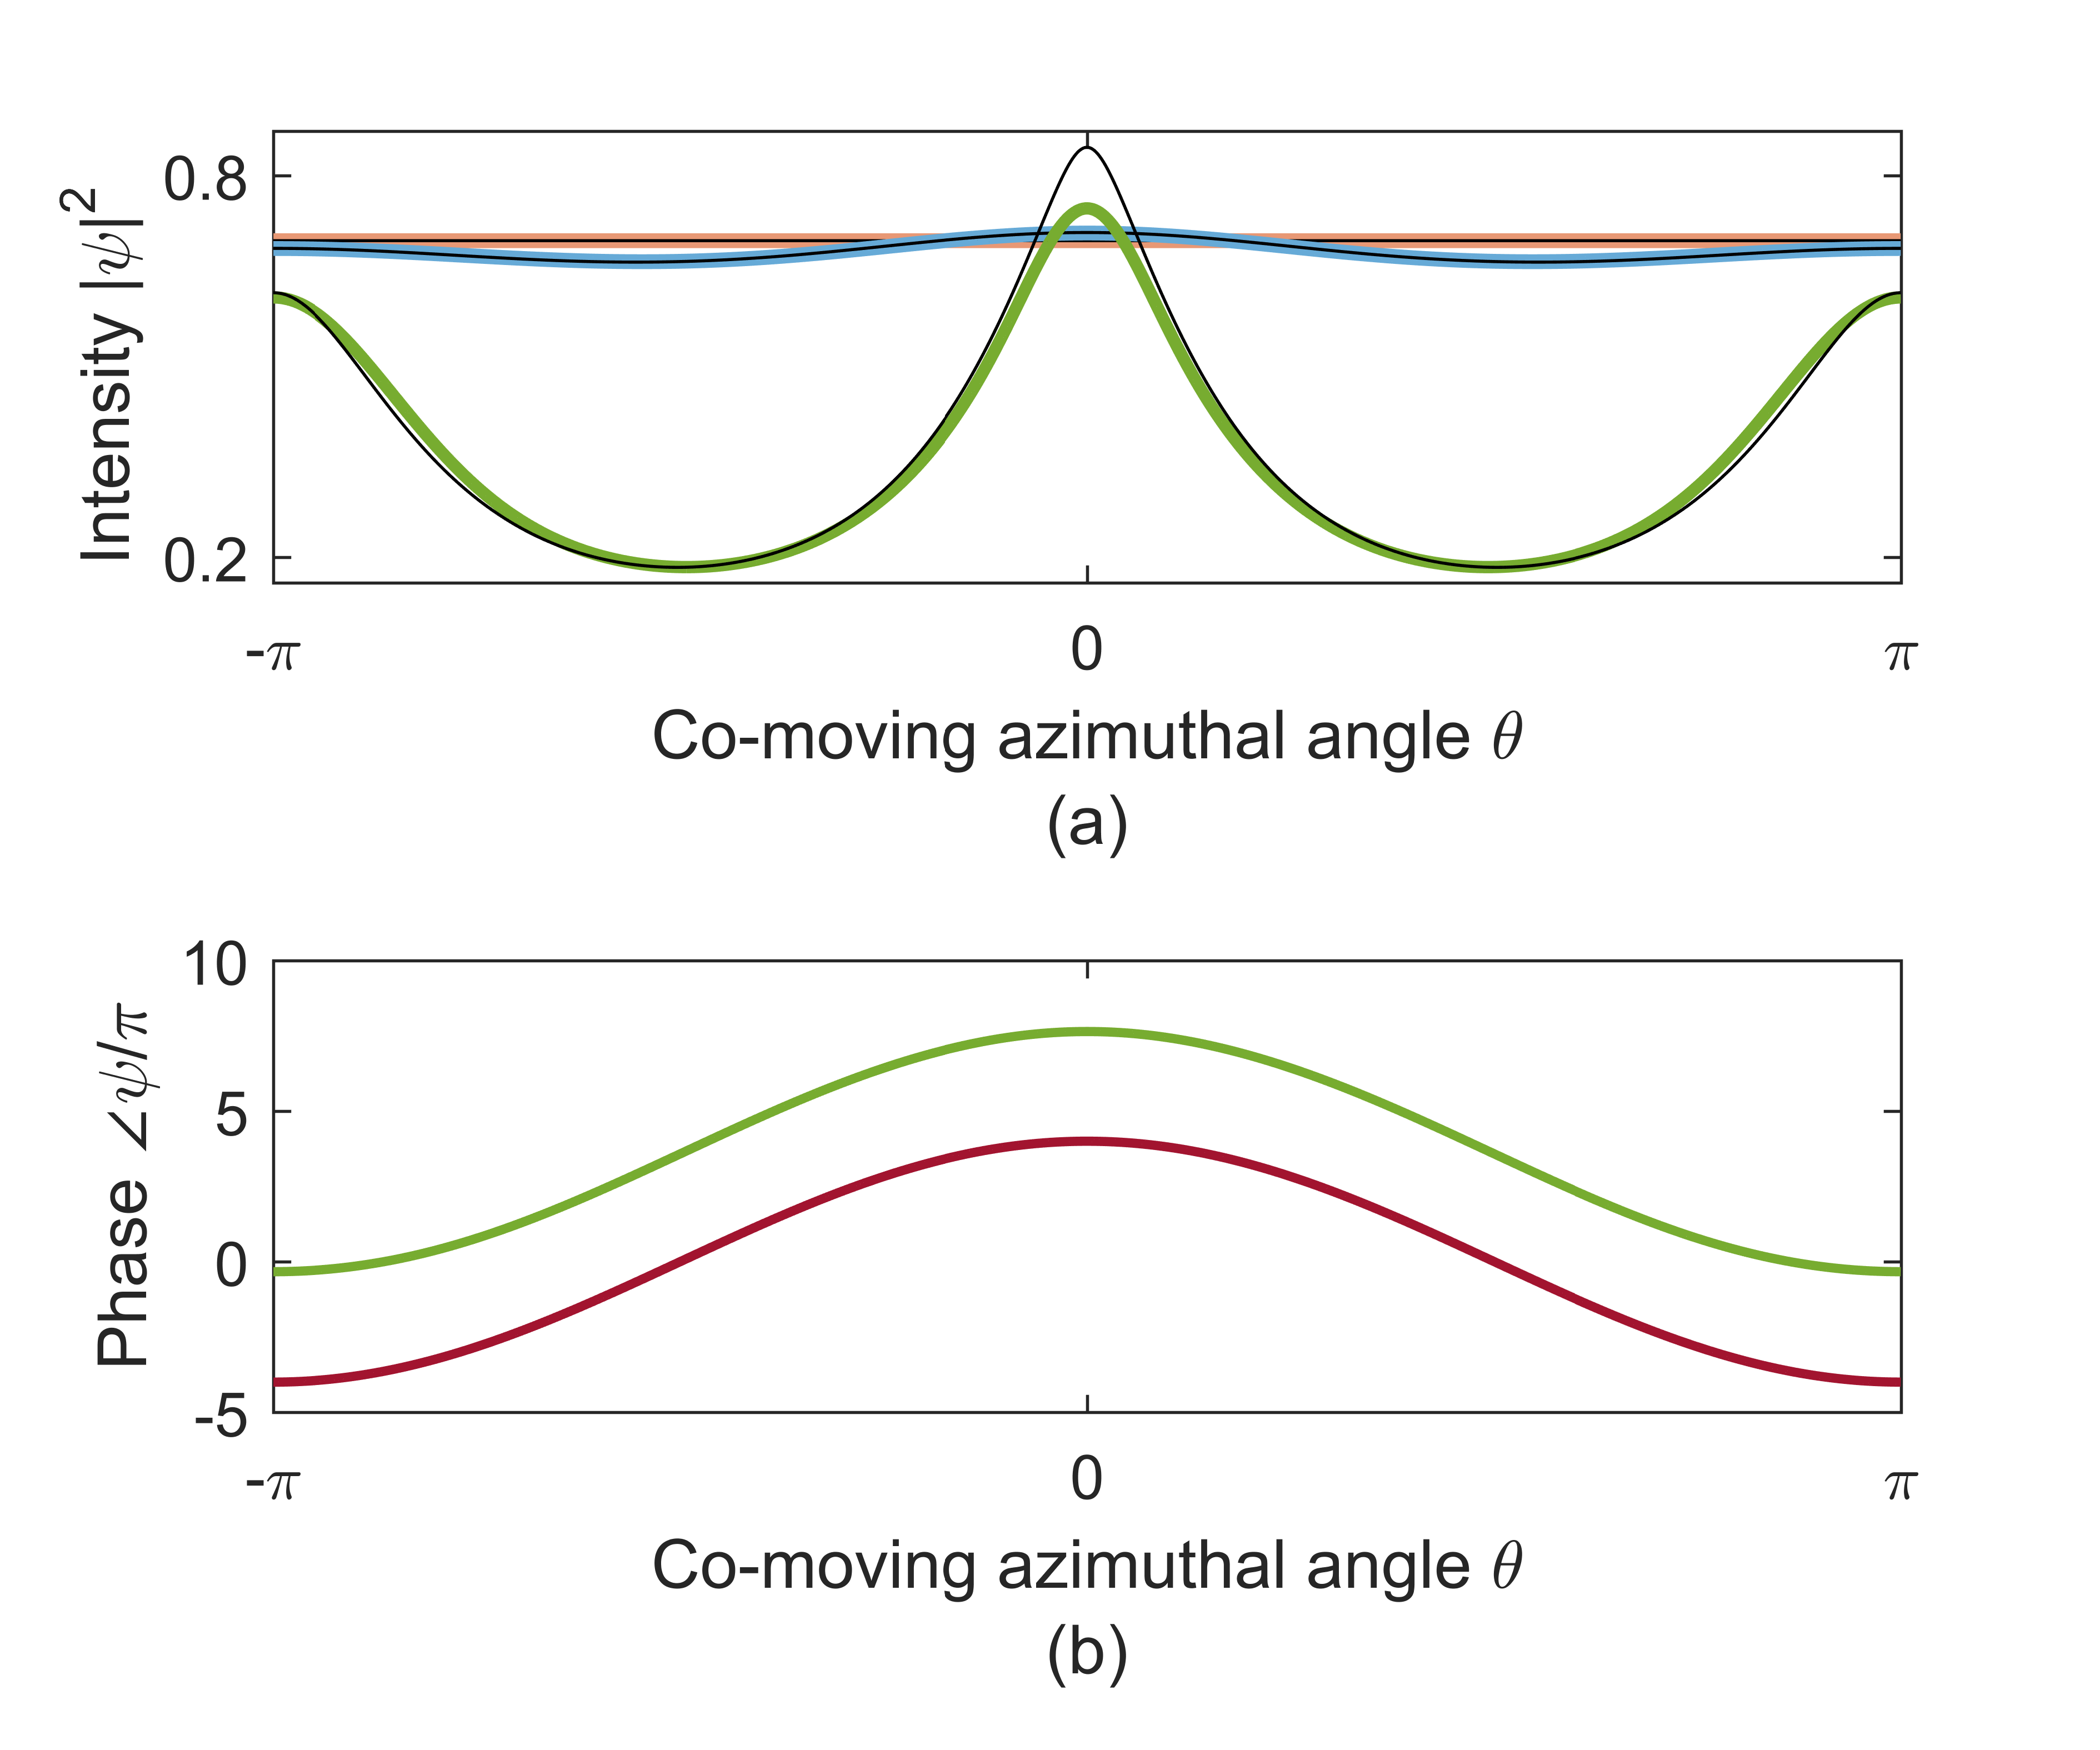
\includegraphics{\FigPath/Figures/PMPumping/PM_background.png}
	\end{center}
	\caption[Quasi-CW background in a PM-pumped resonator]{\textbf{Quasi-CW background in a PM-pumped resonator.} (a) Simulated intensity of the background in the resonator without (orange) and with PM of depth $\delta_{PM}=\pi/2$ (blue) and $\delta_{PM}=4\pi$ (green), with analytical approximations in black. Here $\alpha$ is slightly larger than the critical value for soliton formation. (b) Phase profile of the field $\psi$ corresponding to the green trace in (a) with $\delta_{PM}=4\pi$, and the phase profile of the driving term $Fe^{i\delta_{PM}\cos{\theta}}$ (red) with modulation depth $4\pi$. The phase of the field is very nearly the phase of the drive plus a constant offset.}
	\label{fig:PMbackground}
\end{figure} 

Fig. \ref{fig:PMbackground} shows the predictions of simulations of Eq. \ref{eq:PMLLE} (color) and the analytical model Eq. \ref{eq:PMLLEstat2} (black). The two agree quantitatively for weak modulation ($\delta_{PM}=\pi/2$, blue) and qualitatively with larger depth ($\delta_{PM}=4\pi$, green); both indicate that the field $\psi$ exhibits amplitude variations due to the spatially-varying effective loss and detuning. This phenomenon suggests an explanation for the spontaneous formation of a single soliton as the detuning $\alpha$ is decreased in terms of the local disappearance of Kerr bistability.


\begin{figure}[htpb]
	\begin{center}
		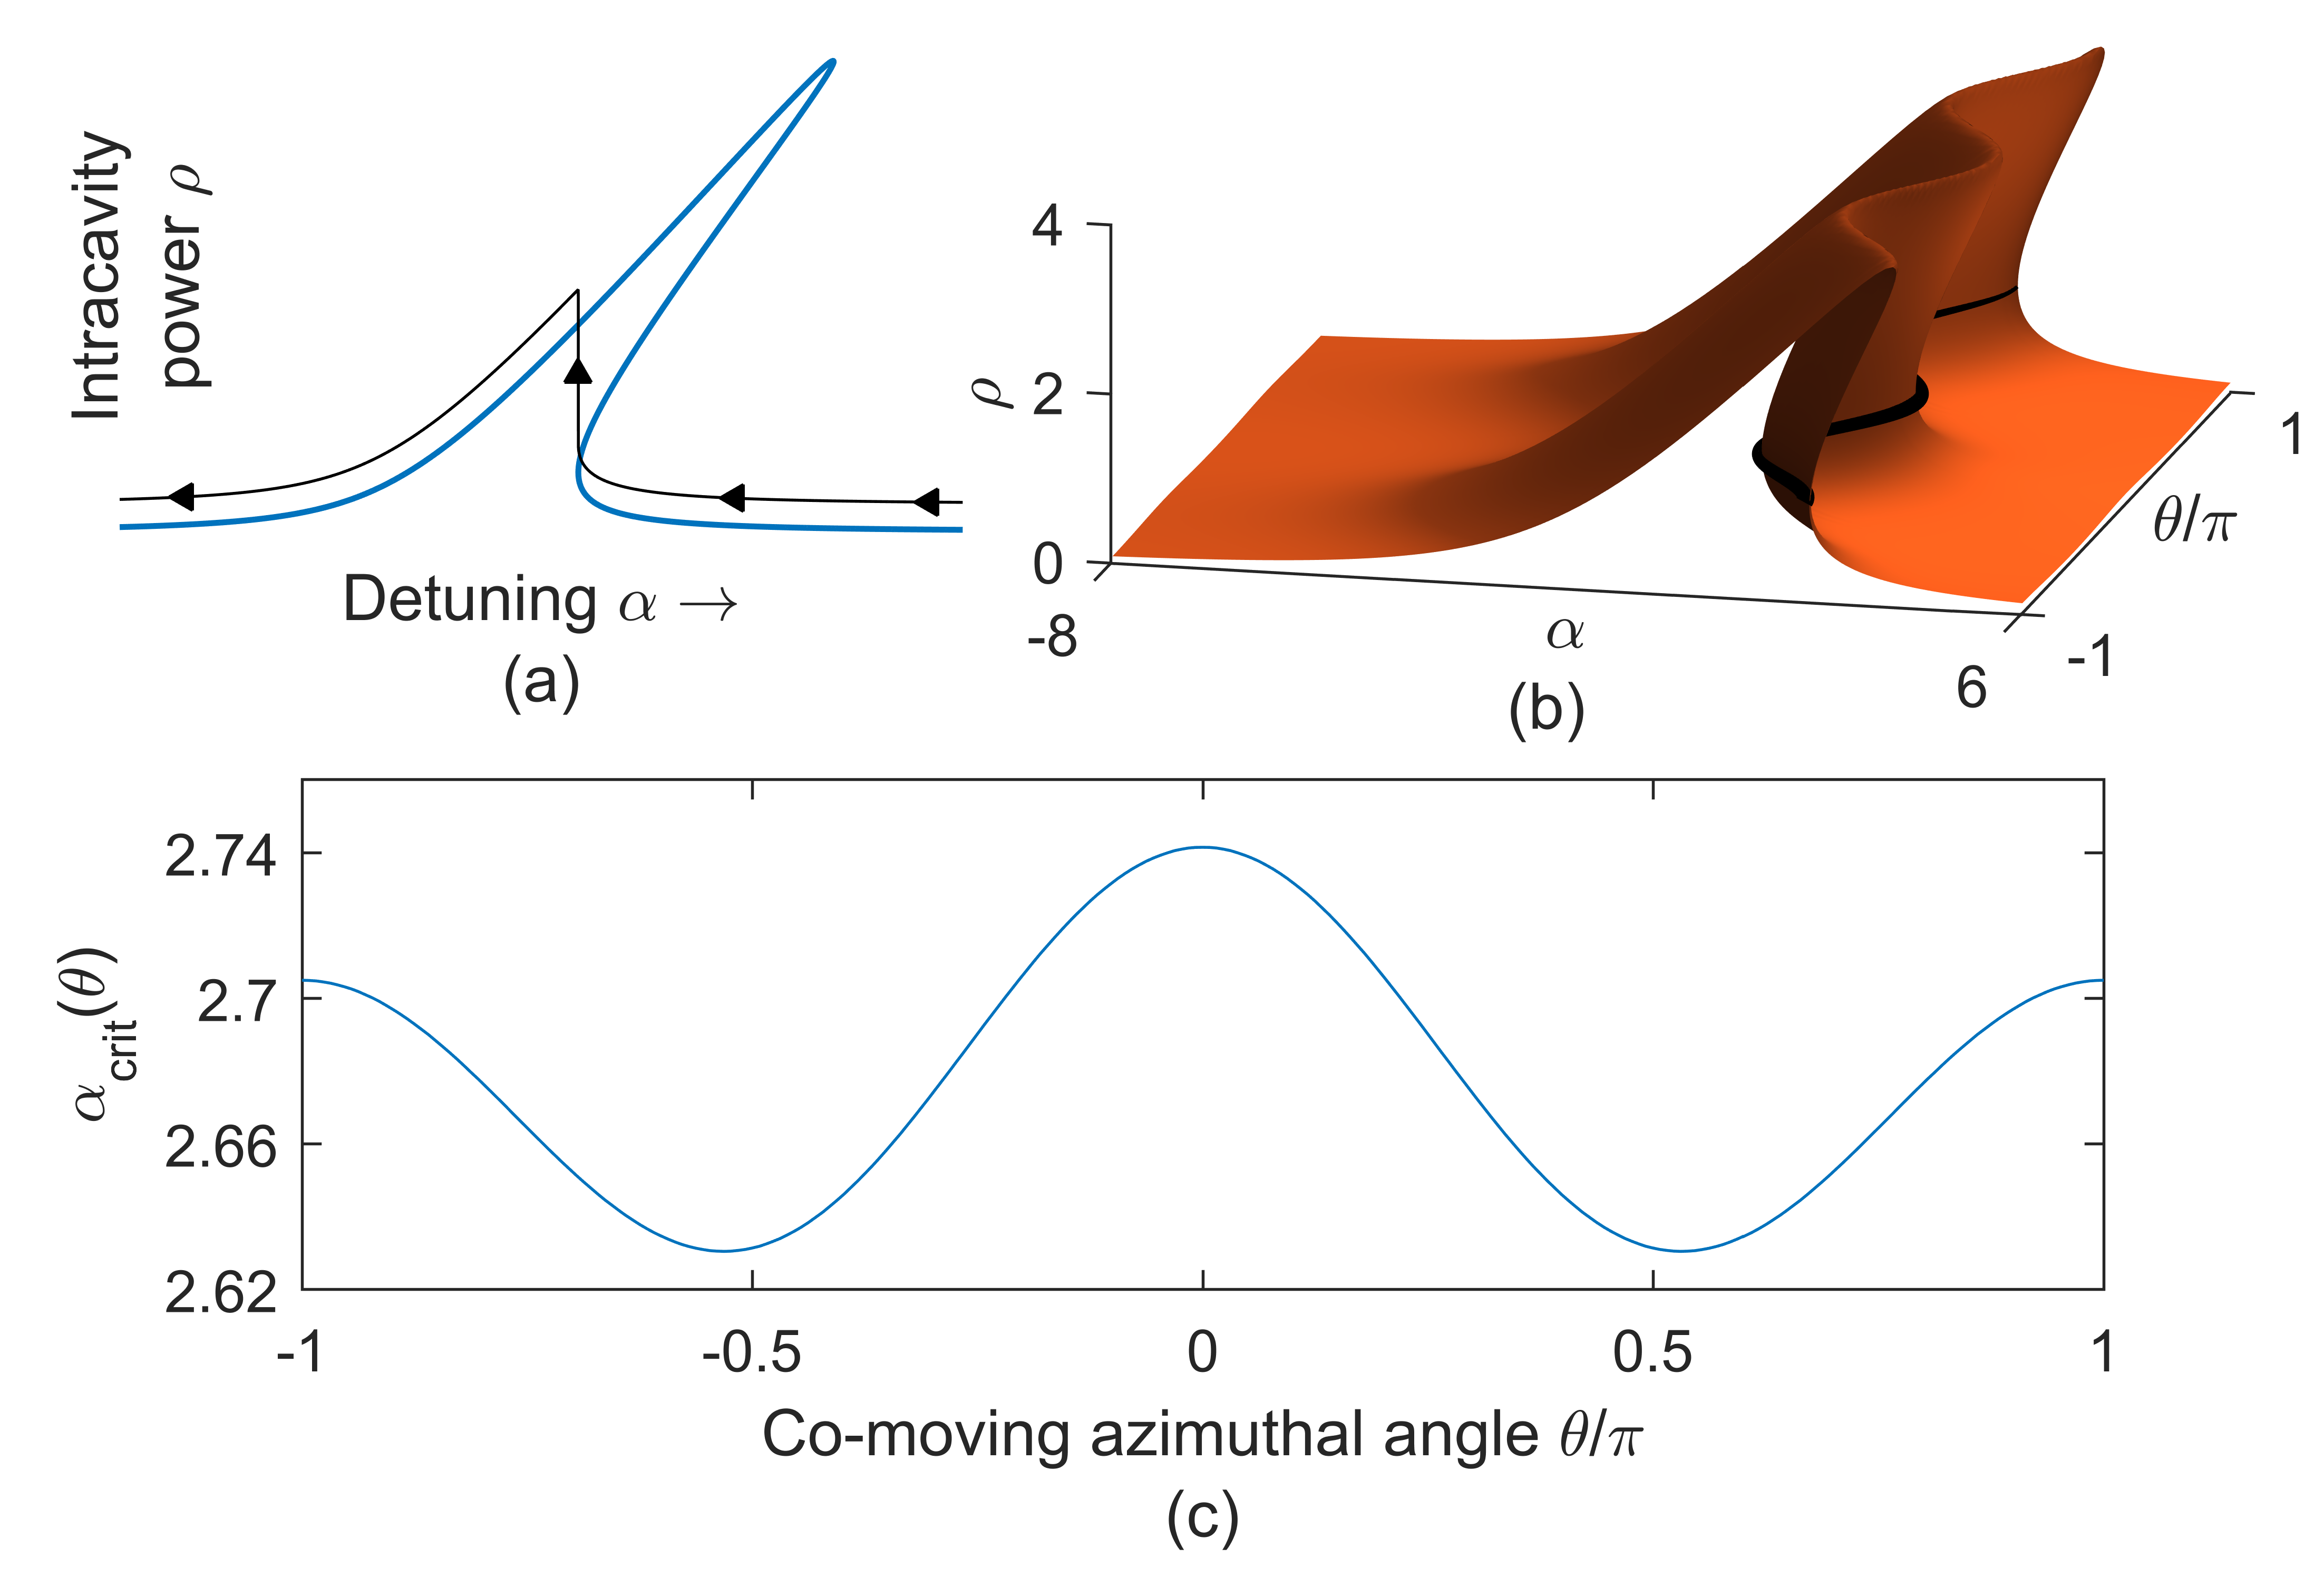
\includegraphics{\FigPath/Figures/PMPumping/PMalphacritWresWmanifold.png}
	\end{center}
	\caption[Mechanism for soliton generation with a PM pump]{\textbf{Mechanism for soliton generation with a PM pump.} (a) Plot of a Kerr-shifted resonance, here with $F^2$=12. The CW background field $\psi_{CW}$ follows the black curve in an increasing-frequency scan of the pump laser (although actually a portion of the upper branch is unstable due to modulation instability above threshold). (b) For the case of a phase-modulated pump, the field $\psi_s(\theta)$ at each point $\theta$ lies on a qualitatively similar resonance that is defined locally by $\gamma(\theta)$ and $\eta(\theta$), with the result that a resonance surface emerges. The resonance surface is shown here for $F^2=4$, $\beta_2=-0.0187$, and $d_{PM}=4\pi$, which is chosen to accentuate the $\theta$-dependence. The curve $\alpha_{crit}(\theta)$ is shown in black. (c) A plot of the value $\alpha_{crit}(\theta)$ at which the Kerr bistability locally vanishes and the field $\psi_s(\theta)$ must jump to the effectively blue-detuned branch, associated with the vertical transition in (a), for $F^2=4$, $\beta_2=-0.0187$, and $\delta_{PM}=\pi$. The value $\alpha_{crit}(\theta=0)$ can be used to approximate the detuning at which a soliton is generated in an increasing-frequency scan of the pump laser; the input parameters here match the level diagram in Fig. \ref{fig:PMenergylevels}.}
	\label{fig:PMalphacrit}
\end{figure} 


As discussed in Sec. \ref{sec:MRanalyticalcurves}, for the LLE with a CW pump the background field $\psi_{CW}$ can take one of two stable values over a range of the parameters $\alpha$ and $F^2$. This leads to the emergence of a tilted resonance lineshape like the one shown in Fig. \ref{fig:PMalphacrit}a, with an effectively red-detuned branch lying at higher values of $\alpha$, an effectively blue-detuned branch lying at lower values of $\alpha$, and an interval in $\alpha$ over which they both exist and the system is bistable (recall that the middle branch is unstable). With spatially-varying effective loss and detuning terms, the field $\psi_s(\theta)$ described by Eq. \ref{eq:PMLLEstatpsi} now takes a value at each point in the cavity that is determined by the local parameters $\gamma(\theta)$ and $\eta(\theta)$, with the result that each point lies on its own effective resonance. The resulting resonance \textit{surface} is shown in Fig. \ref{fig:PMalphacrit}b. It can be independently determined for each point in the cavity whether $\psi_s(\theta)$ exhibits bistability. Applying the analysis presented in Sec. \ref{sec:MRanalyticalcurves} to Eq. \ref{eq:PMLLEstat2}, we identify the value of $\rho$ associated with the disappearance of the bistability in a decreasing-$\alpha$ scan as the smaller value $\rho_-$ at which $\partial F^2/\partial\rho=0$:
\begin{equation}
\rho_-=\left(2\eta-\sqrt{\eta^2-3\gamma^2}\right)/3,
\end{equation}
For fixed $F^2$ the function $\alpha_{crit}(\theta)$ describing the critical value of $\alpha$ at which the bistability ends is found by numerically solving the implicit equation for $\alpha_{crit}$ obtained by inserting $\rho_-$ into Eq. \ref{eq:PMLLEstat}:
\begin{equation}
F^2=\left[\gamma^2(\theta)+\left(\eta(\theta)-\rho_-(\theta)\right)^2\right]\rho_-(\theta),
\end{equation}
where $\alpha_{crit}(\theta)$ is included via $\eta(\theta)=\alpha_{crit}(\theta)-\frac{\beta_2}{2}\delta_{PM}^2\sin^2{\theta}$. Fig. \ref{fig:PMalphacrit}c shows a calculation of $\alpha_{crit}(\theta)$ for $F^2=4$ and $\beta_2=-0.0187$, which is chosen to match the dispersion of the resonator used for the experiments presented below. For $\theta=0$ this calculation predicts disappearance of the bistability, and subsequent soliton generation, at $\alpha=2.741$, which is a difference of 0.4 \% from the value $\alpha=2.729$ observed in the simulation presented in Fig. \ref{fig:PMenergylevels}. The same calculation predicts disappearance of the bistability for $\theta=\pi$, at which point a second soliton is generated, at $\alpha=2.705$, which is also in close agreement with the simulation.



%\begin{figure}[htpb]
%	\begin{center}
%		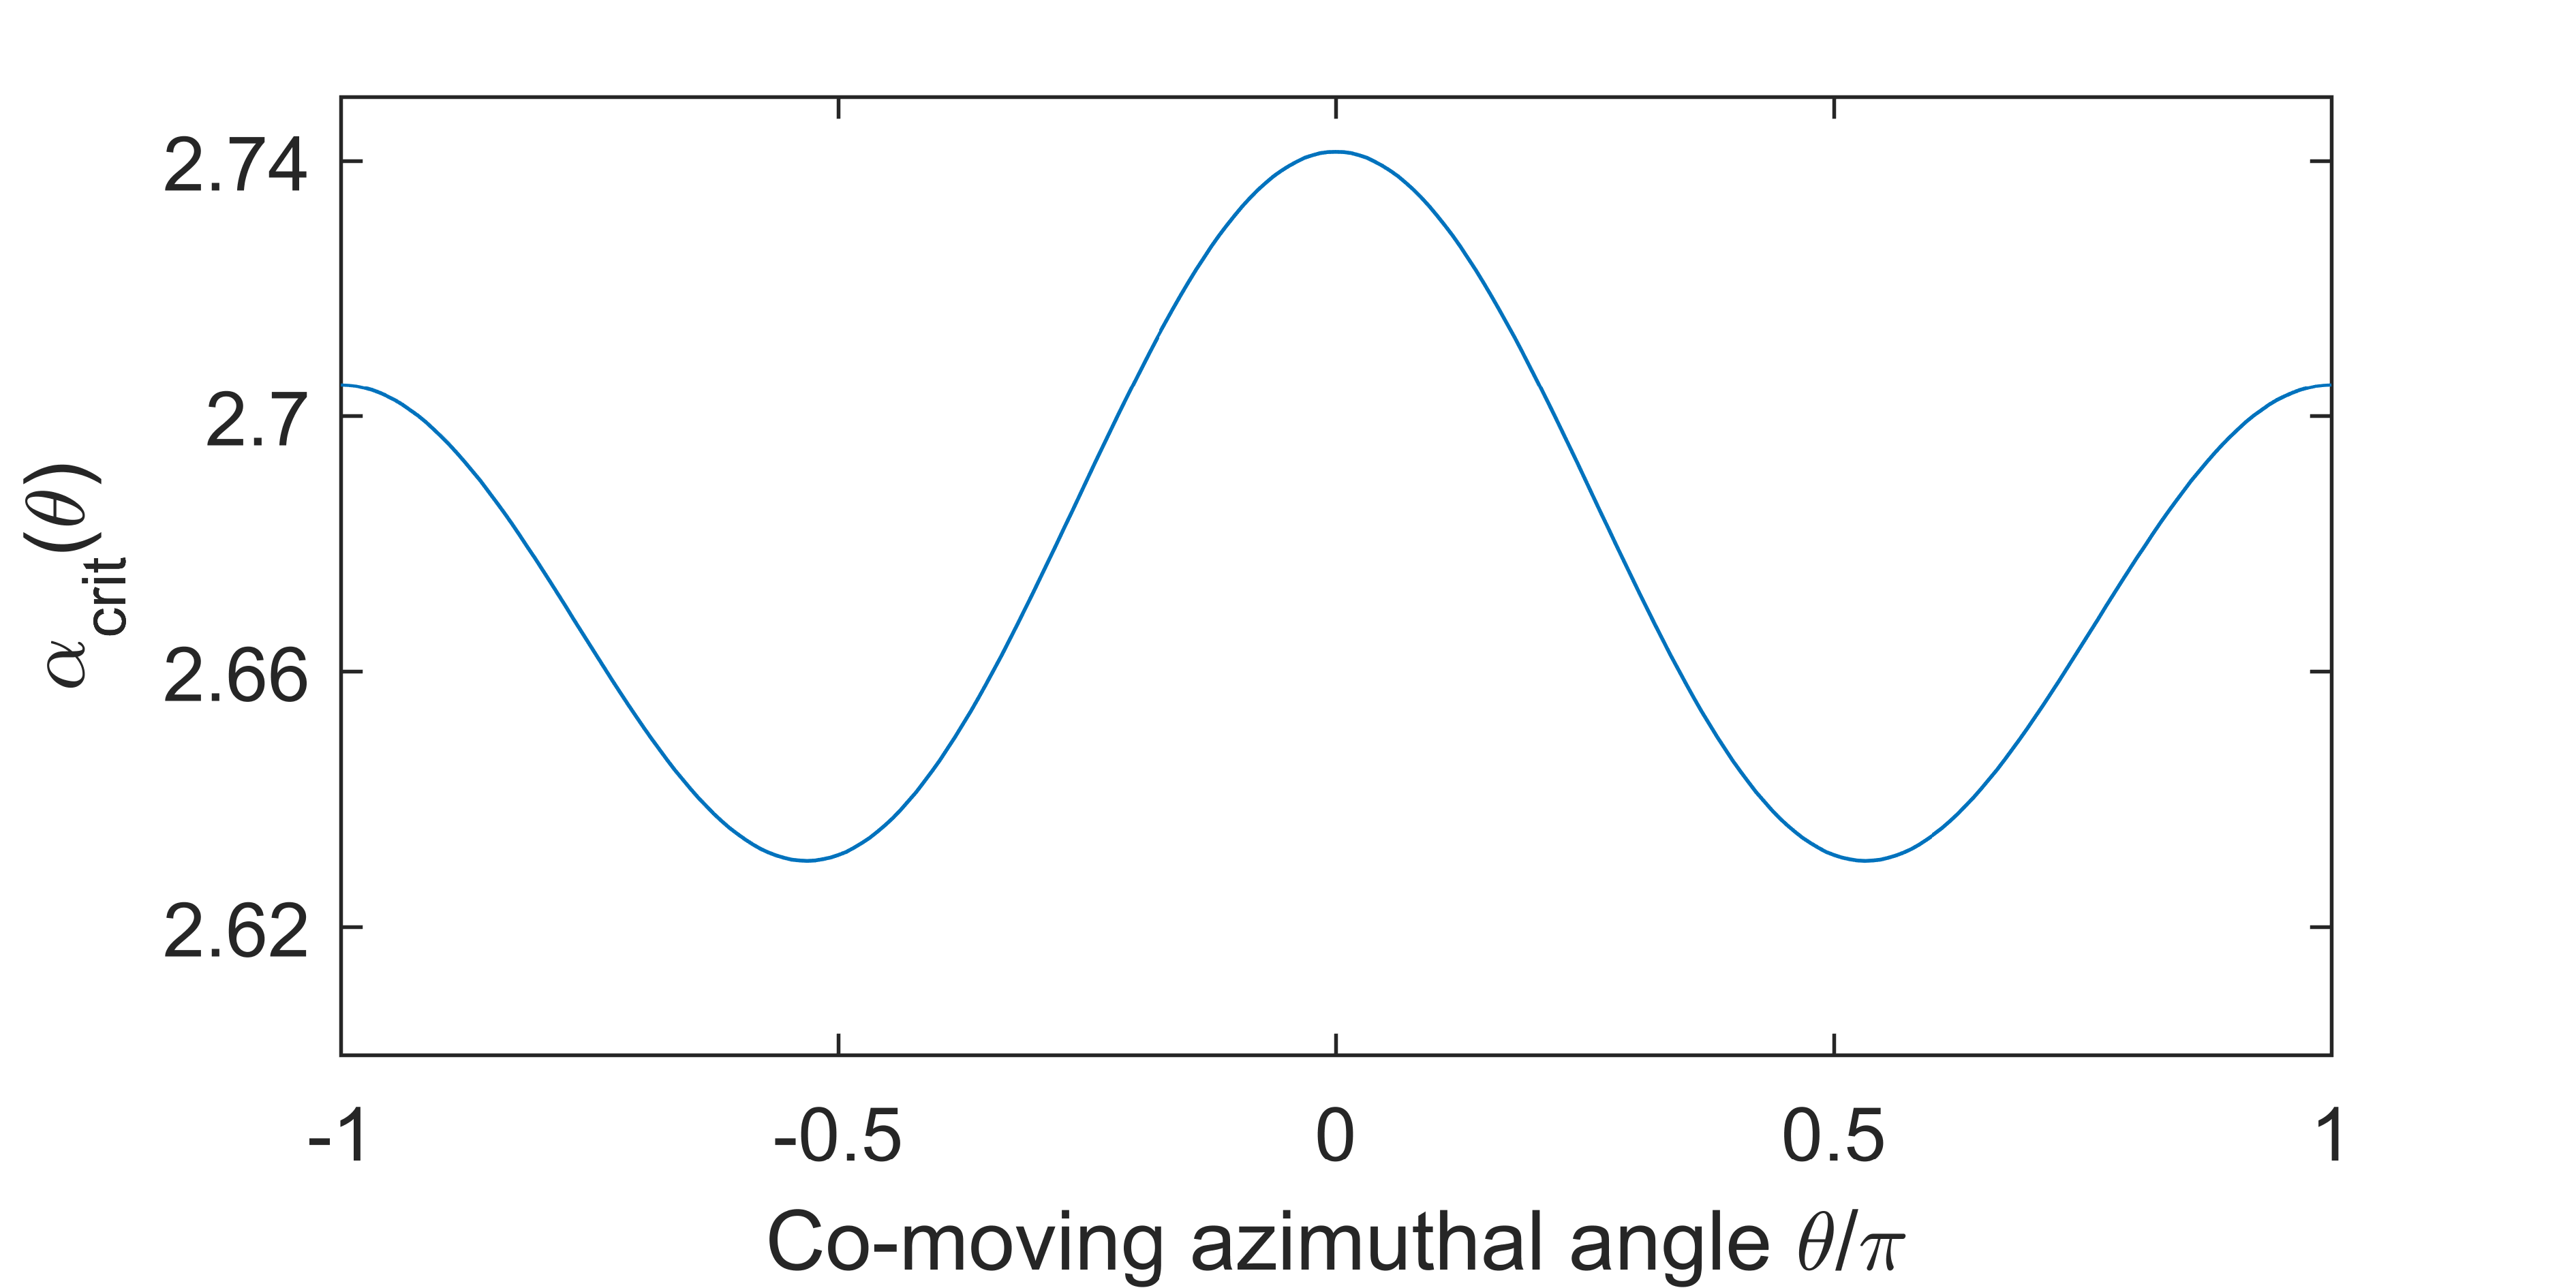
\includegraphics{\FigPath/Figures/PMPumping/PMalphacrit.png}
%	\end{center}
%	\caption[Critical values of $\alpha$ for the disappearance of Kerr bistability]{\textbf{Critical values of $\alpha$ for the disappearance of Kerr bistability.} A plot of the value $\alpha_{crit}(\theta)$ at which the Kerr bistability vanishes \textit{locally} and the system must locally jump to the effectively blue-detuned branch. This plot is generated with $F^2=$, $\beta=-0.0187$. The value $\alpha_{crit}(\theta=0)$ can be used to approximate the detuning at which a soliton is generated in an increasing-frequency scan of the pump laser.}
%	\label{fig:PMalphacrit}
%\end{figure} 

%\begin{figure}[htpb]
%	\begin{center}
%		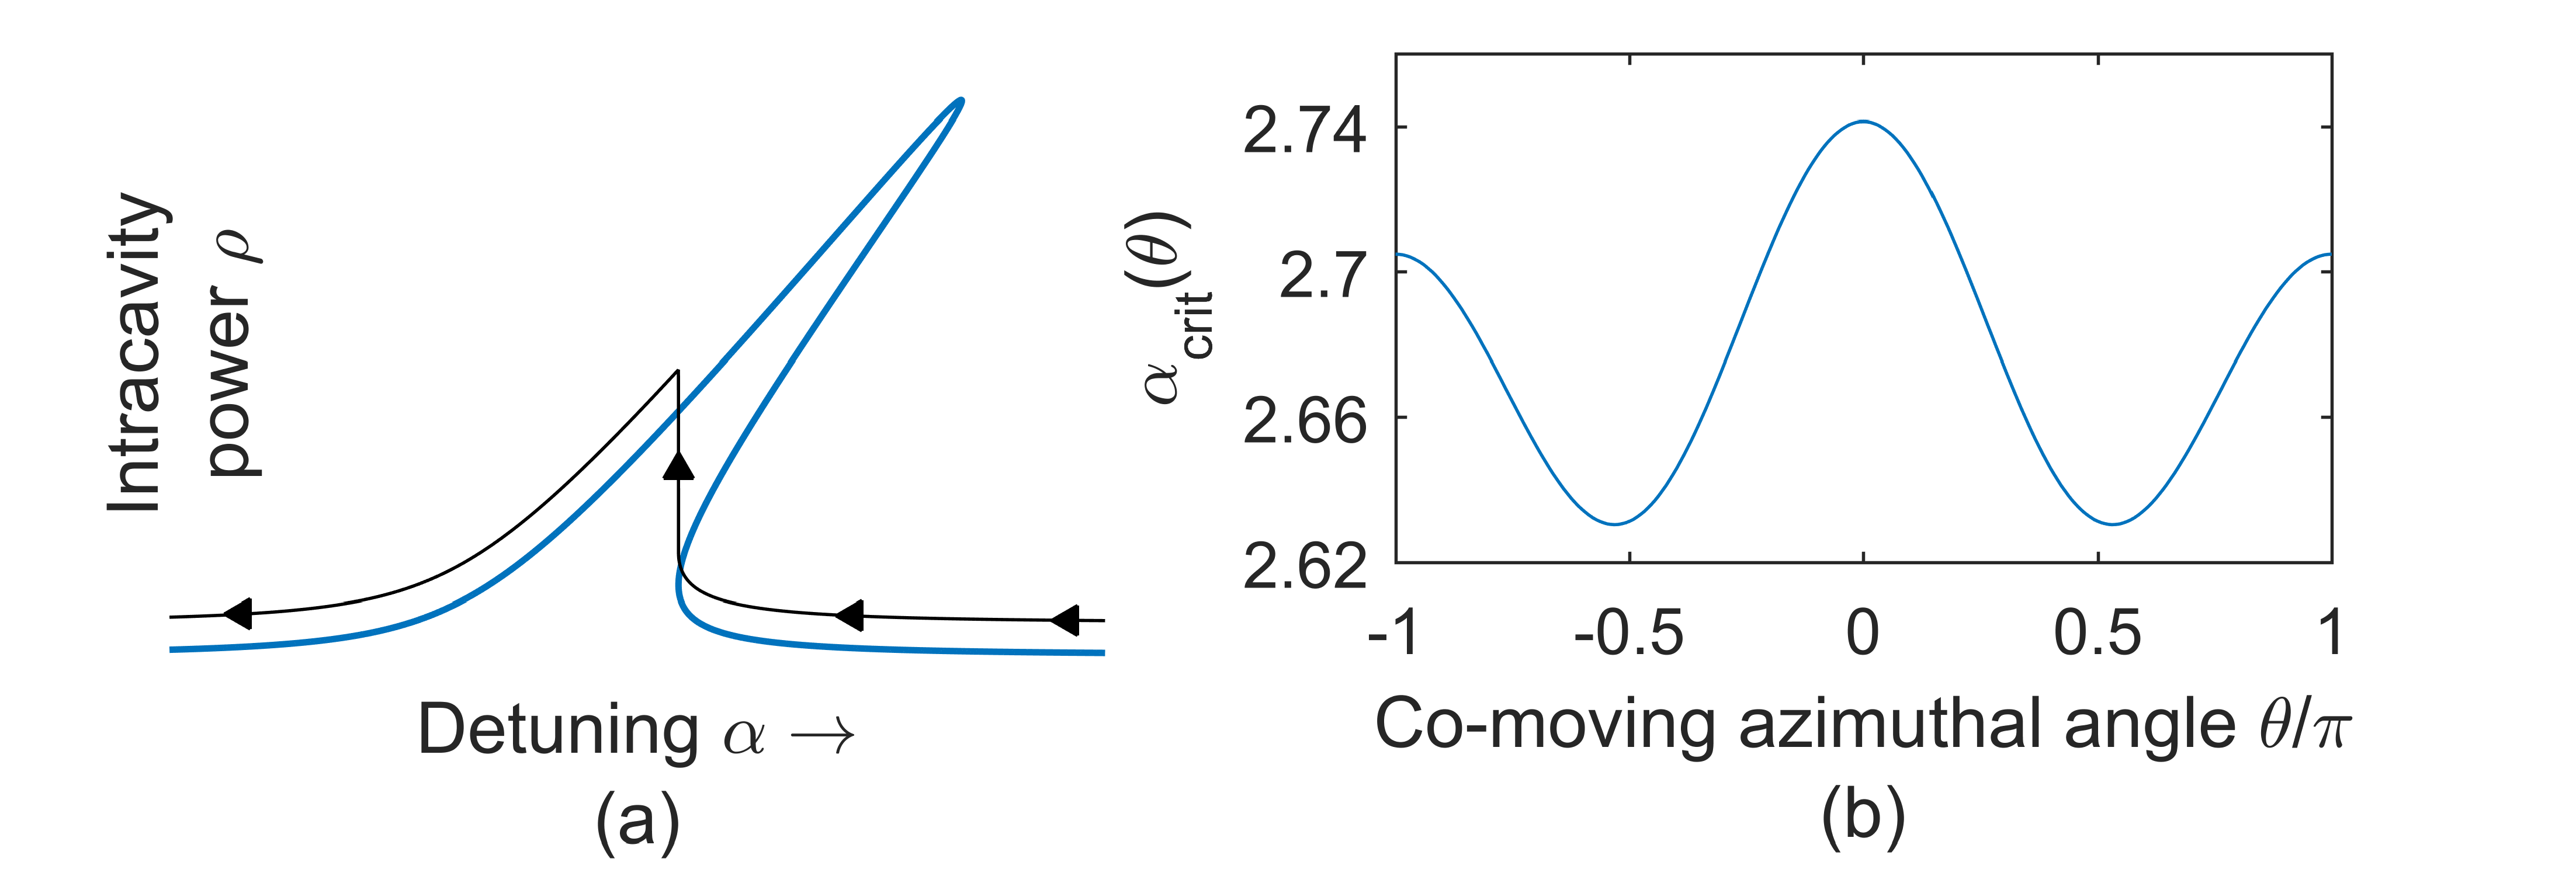
\includegraphics{\FigPath/Figures/PMPumping/PMalphacritWres.png}
%	\end{center}
%	\caption[Mechanism for soliton generation with a PM pump]{\textbf{Mechanism for soliton generation with a PM pump.} (a) Plot of a Kerr-shifted resonance, here with $F^2$=12. The CW background field $\psi$ follows the black curve in an increasing-frequency scan of the pump laser. For the case of a phase-modulated pump, the field $\psi_s(\theta)$ lies at a point on a qualitatively similar resonance that is defined locally by $\gamma(\theta)$ and $\eta(\theta$) for each point $\theta$ in the co-moving frame. (b) A plot of the value $\alpha_{crit}(\theta)$ at which the Kerr bistability locally vanishes and the field $\psi_s(\theta)$ must jump to the effectively blue-detuned branch, associated with the vertical transition in (a). This plot is generated with $F^2=4$, $\beta=-0.0187$. The value $\alpha_{crit}(\theta=0)$ can be used to approximate the detuning at which a soliton is generated in an increasing-frequency scan of the pump laser.}
%	\label{fig:PMalphacrit}
%\end{figure} 



%These parameters determine whether the quasi-CW background locally exhibits the bistability that is well-known in the case of a CW pump laser [18,21], which suggests a mechanism for spontaneous single-soliton generation: as α is decreased, the stable effectively red-detuned branch of the resonance locally vanishes at the peak of the quasi-CW background, leading to the formation of a soliton. By following the analysis in e.g. Ref.  [18] (Eqs. 11-14), we can approximate the value of α where this occurs at θ=0; for the diagram shown in Fig. 1b this predicts soliton generation at α=2.741, in excellent agreement (0.4 % error) with the value α=2.729 obtained in numerical simulations. 
%
%Fig.  compares the predictions of numerical LLE simulations (color) with the analytical model (black). The two agree quantitatively at small modulation depth () and qualitatively at larger depth . Both the simulations and the approximate analytical solution indicate that the background has two peaks per round trip in the presence of phase modulation, which suggests a mechanism for spontaneous single-soliton generation: \todo{update this} At threshold the larger peak becomes locally unstable, and a soliton is formed by local modulation instability \cite{Ceoldo2016,Wang2018}. Moreover, it is known that if solitons exist elsewhere they are pushed to the larger peak by the background’s modulated phase \cite{Jang2015a}. This makes superpositions of $N>1$ solitons unstable and practically forbidden. Generation of single solitons then simply requires tuning the pump power and frequency to appropriate values, regardless of initial conditions. 
%
%The detuning for soliton generation can be estimated using Eq. \ref{eq:PMLLEstat} by calculating the value of $\alpha$ where $\rho(\theta=0)=1$. This comes with a further approximation, as simulations reveal that the critical detuning for soliton formation is near but not necessarily at $\rho=1$ because the spatial interval over which threshold is exceeded must have some minimum width. However, this approach quantitatively captures the behavior shown in Fig. \ref{fig:PMenergylevels}, predicting soliton generation at $\alpha=2.737$.

\section{Spontaneous generation of single solitons using a phase-modulated pump laser}


We demonstrate deterministic generation of single solitons without condensation from an extended pattern in a 22-GHz FSR silica microdisk resonator. This resonator has $\Delta\nu\sim$ 1.5 MHz linewidth, and was fabricated using a chemical etching process at CalTech \cite{Lee2012}. We generate a frequency-agile laser for pumping the resonator by passing a CW seed laser through a single-sideband modulator (SSB) that is driven by a voltage-controlled oscillator (VCO) \cite{Stone2017}. The seed laser is extinguished in the modulator and the resulting sideband can be swept by adjusting the voltage applied to the VCO; sweeping rates up to 100 GHz/$\mathrm{\mu}$s over a range over 4 GHz are possible. The pump laser is phase-modulated with index $\delta_{PM}\sim\pi$ and amplified to normalized power $F^2$ between 2 and 6. The pump-laser detuning $\nu_0-\nu_{p}$, where $\nu_0$ is the frequency of the pumped mode and $\nu_p$ is the frequency of the pump laser, is measured in real time using an AOM-shifted probe beam as shown in Fig. \ref{fig:PMsetup}, and the high-bandwidth feedback allowed by the VCO/SSB scheme allows thermal instabilities associated with the red detuning that is required for soliton generation to be overcome. 

\begin{figure}[htpb]
	\begin{center}
		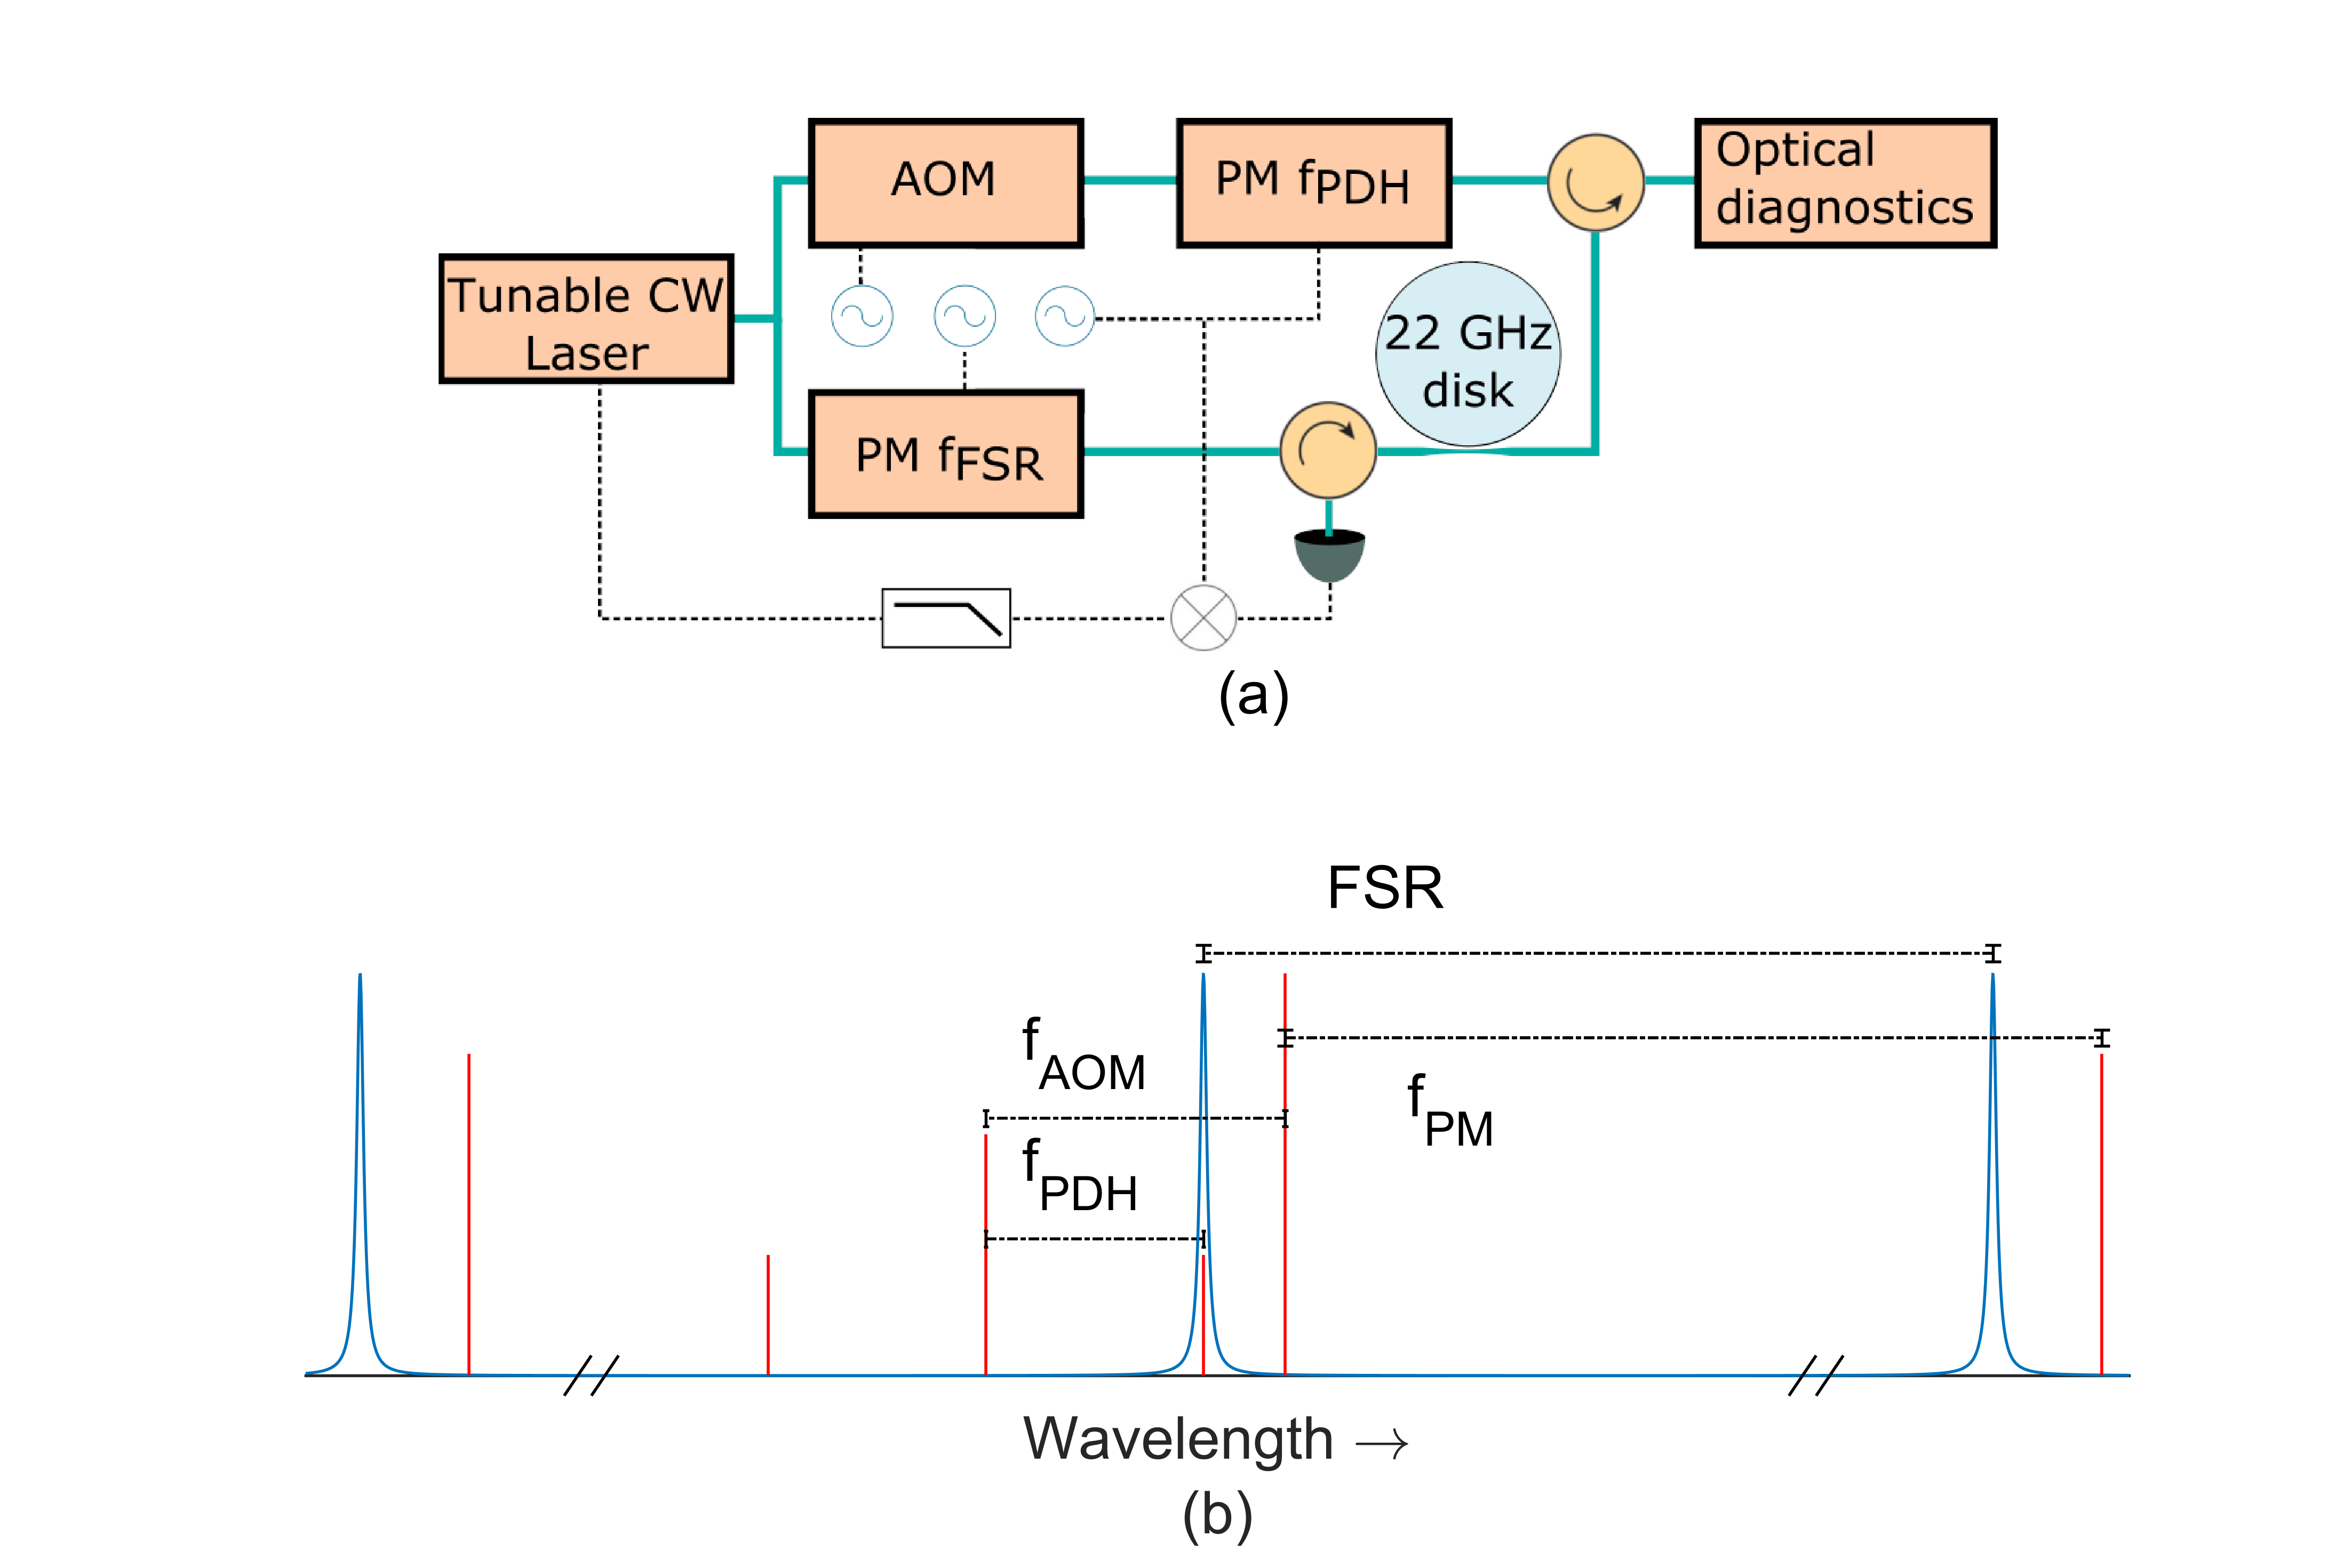
\includegraphics{\FigPath/Figures/PMPumping/PMsetup.png}
	\end{center}
	\caption[Experimental setup for soliton generation with a phase-modulated pump laser]{\textbf{Experimental setup for soliton generation with a phase-modulated pump laser.} (a) Schematic diagram of the experimental setup, including the pump laser phase-modulated at frequency $f_{PM}\sim f_{FSR}$ and an AOM-shifted probe beam that is modulated at frequency $f_{PDH}$ for implementation of a Pound-Drever-Hall sideband lock. The probe beam addresses the resonator in the counter-propagating direction. (b) Frequency-domain diagram of the scheme used to maintain stable red detuning of the pump laser. As $f_{PDH}$ is increased, the detuning $\alpha$ is decreased.}
	\label{fig:PMsetup}
\end{figure} 


To generate single solitons, we begin with large red detuning $\nu_0-\nu_{p}=$40 MHz and decrease the detuning until a soliton is generated near $\nu_0-\nu_{p}\sim$5 MHz detuning; this value depends on the pump power and coupling condition. We measure the power converted by the Kerr nonlinearity to new frequencies by passing a portion of the resonator's output through an optical band-reject filter that attenuates the power at frequencies corresponding to the phase-modulated pump laser. This `comb power' measurement reveals a step upon soliton formation, as shown in Fig. \ref{fig:PMgen}a, after which we can measure the soliton spectrum with phase-modulation sidebands on the pump shown in Fig. \ref{fig:PMgen}b. After soliton generation, we observe that the soliton can be preserved while the detuning is increased again, consistent with Fig. \ref{fig:PMenergylevels}. Additionally, we observe that it is possible to turn off the phase modulation without loss of the soliton, in agreement with the simulations presented in Ref. \citeNoBrackets{Taheri2015}.

Automating soliton generation by repeatedly scanning the laser into resonance ($\nu_0-\nu_{p}\sim$5 MHz) and back out again ($\nu_0-\nu_{p}\sim$20 MHz, far enough that the soliton is lost) has enabled reversible generation of 1000 solitons in 1000 trials over 100 seconds, with a measured 100 $\%$ success rate. Our probe beam allows measurement of the detuning at which soliton generation occurs, which changes little from run to run. We present a histogram of detuning measurements for the generation of 160 solitons in Fig. \ref{fig:PMgen}c. 

\begin{figure}[htpb]
	\begin{center}
		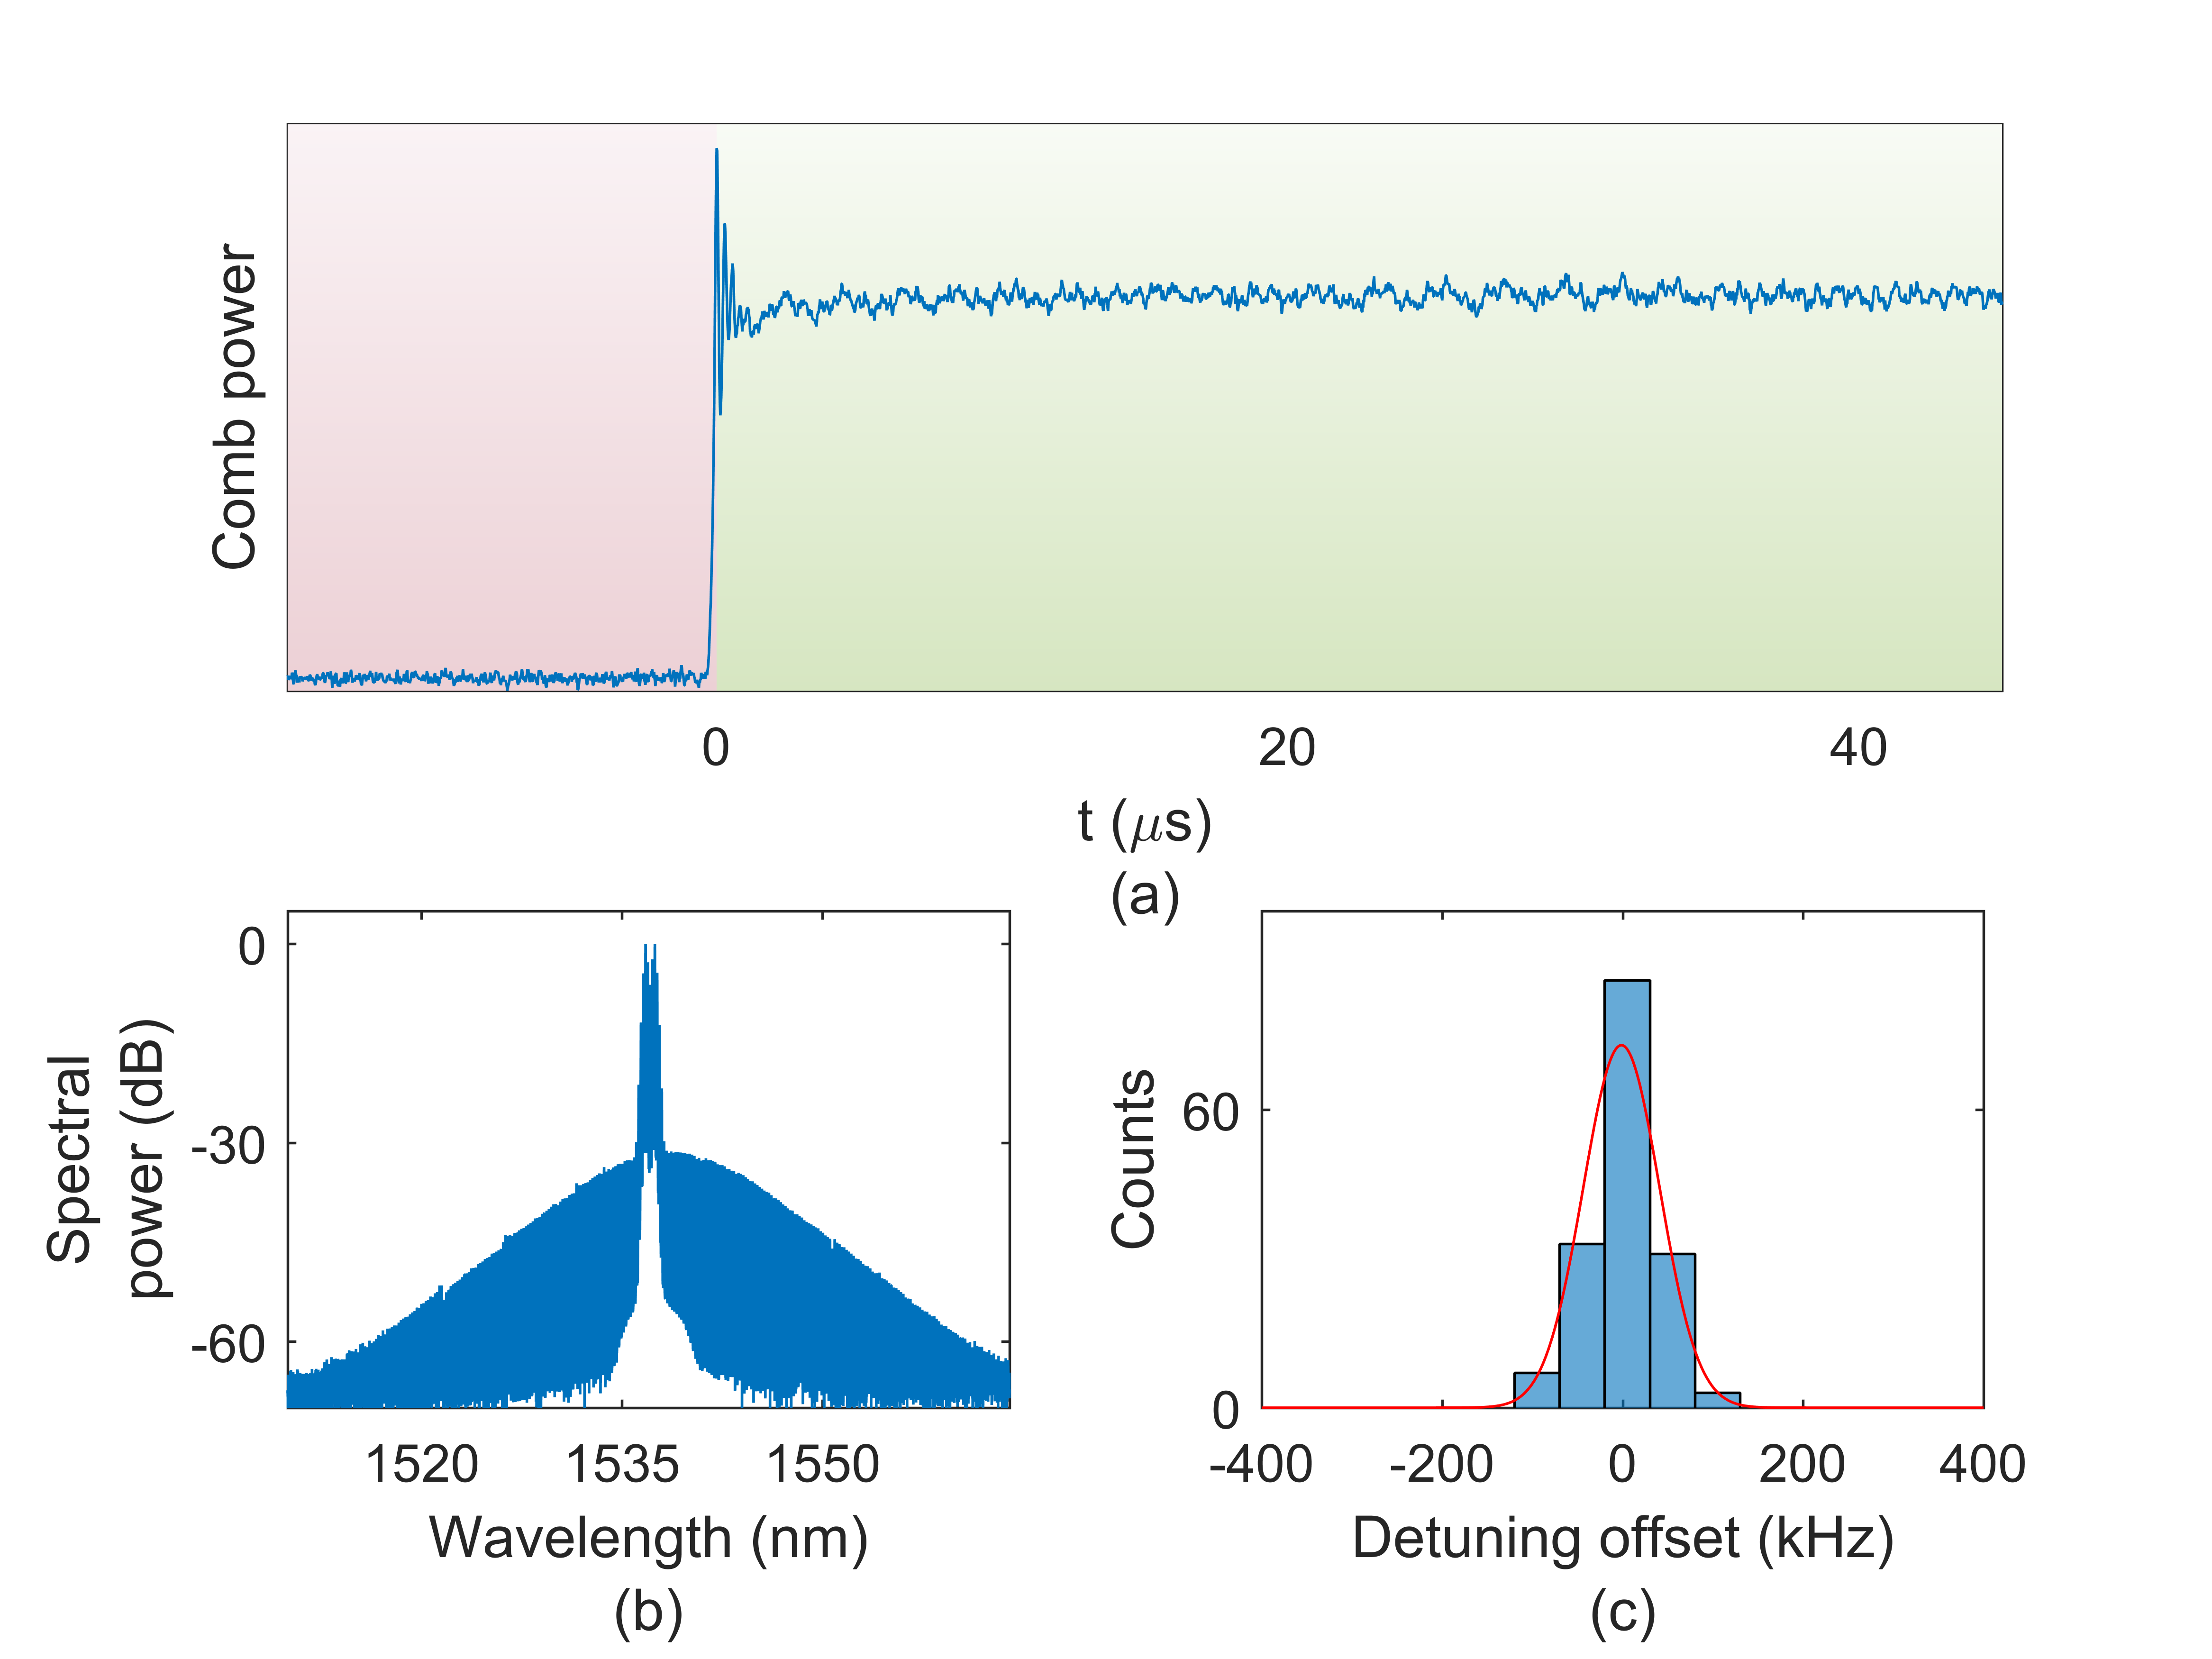
\includegraphics{\FigPath/Figures/PMPumping/PMstepAndSpecAndHist.png}
	\end{center}
	\caption[Spontaneous generation of solitons using a phase-modulated pump laser]{\textbf{Spontaneous generation of solitons using a phase-modulated pump laser.} (a)~`Comb power' trace obtained by filtering the pump laser out of the spectrum of light transmitted past the resonator, indicating a discrete step in the amount of frequency-converted light upon direct generation of a soliton. (b) Optical spectrum of a spontaneously generated soliton. The spectrum of the phase-modulated pump laser is visible as the set of higher-amplitude lines in the center. (c)~Histogram of measured detuning values at which a soliton is generated relative to a reference (mean) value over 160 trials.}
	\label{fig:PMgen}
\end{figure} 

\section{Soliton control using a phase-modulated pump laser}

In addition to enabling deterministic generation of single solitons, phase modulation of the pump laser also facilitates timing and repetition-rate control of the resulting out-coupled pulse train. We characterize this control by measuring the repetition rate of the soliton pulse train as the phase-modulation frequency is varied. This measurement is conducted as follows: First, we photodetect the pulse train after removing the central spectral lines corresponding to the phase-modulated pump laser using an optical band-reject filter. Then, in order to obtain a measurement trace of the repetition rate as a function of time, the photodetected signal is mixed with a local oscillator to reduce the signal frequency from $f_{rep}$ to $\sim$ 1 MHz, after which a spectrogram of the resulting waveform is calculated.

\begin{figure}[htpb]
	\begin{center}
		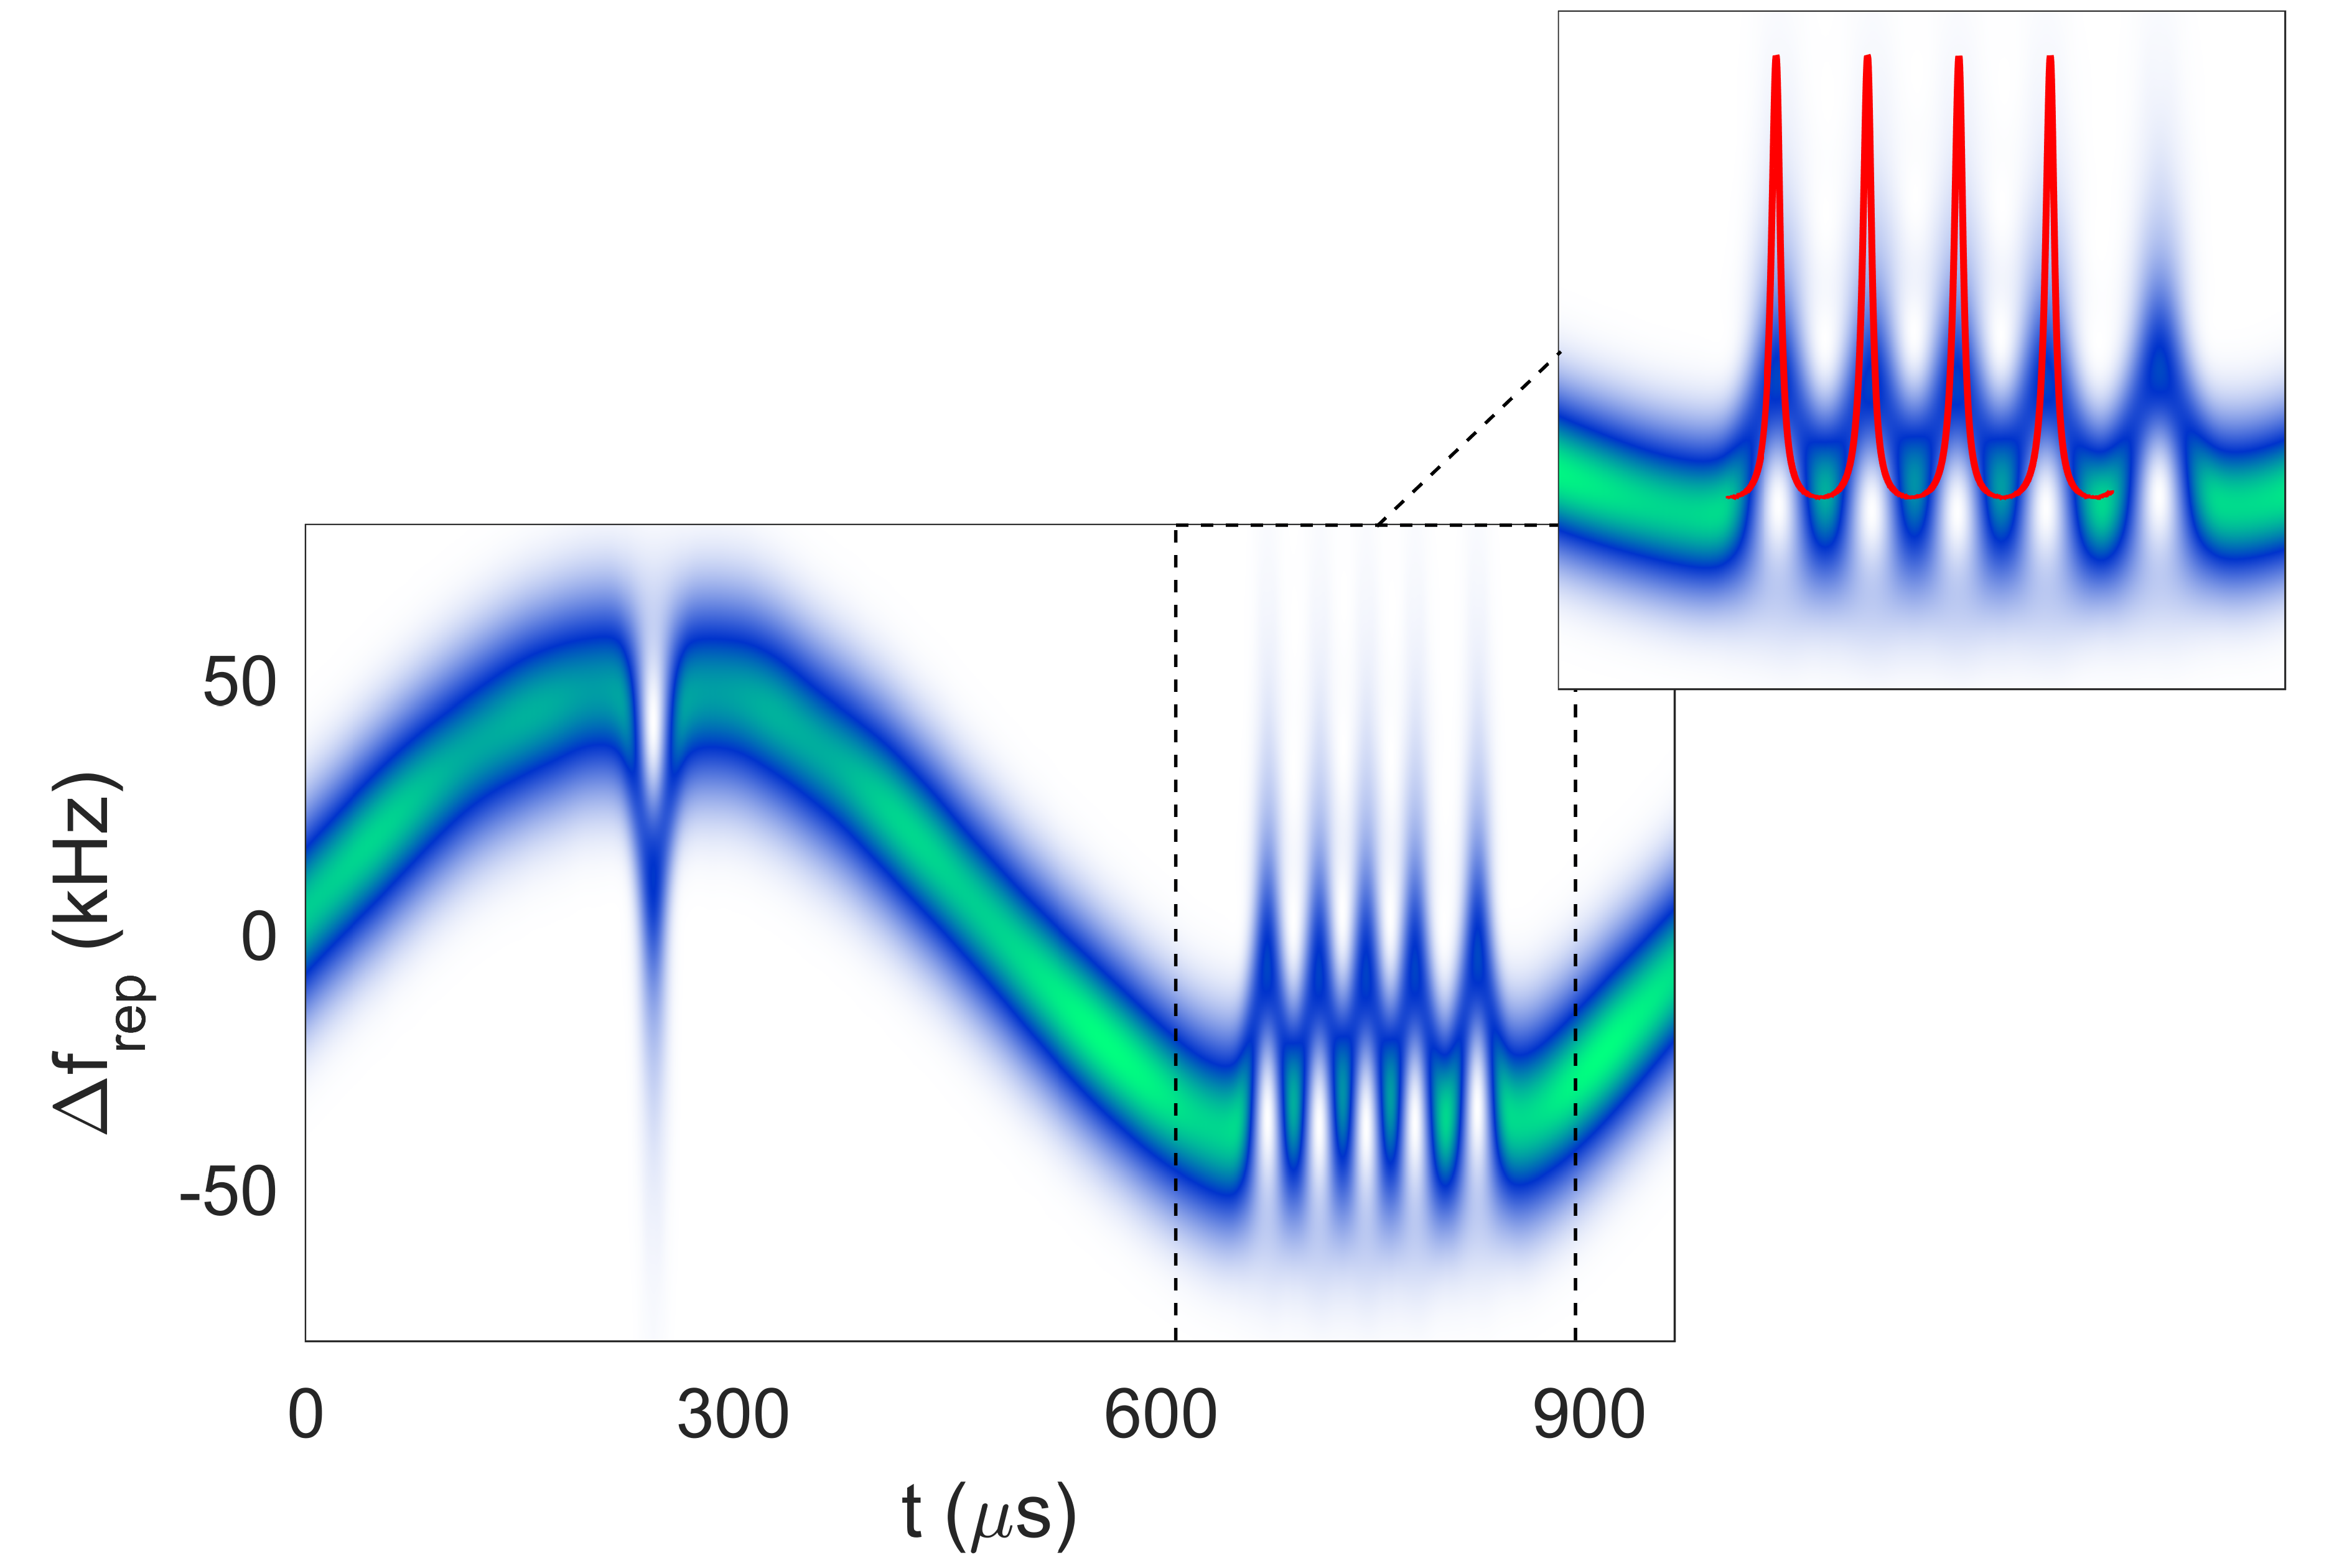
\includegraphics{\FigPath/Figures/PMPumping/PMsweep.png}
	\end{center}
	\caption[Repetition-rate control using a phase-modulated pump laser]{\textbf{Repetition-rate control using a phase-modulated pump laser.} Spectrogram of the measured repetition rate of the soliton pulse train generated by a phase-modulated pump laser as the frequency of phase modulation is swept through $\pm$50 kHz over 1 ms. Glitches in the spectrogram indicate that the range over which $f_{rep}$ can be locked to $f_{PM}$ has been exceeded. Inset: Qualitative agreement with simulations when $f_{PM}$ is outside of the locking bandwidth, shown in red. As the soliton and the pump phase evolve at different frequencies $f_{rep}$ and $f_{PM}$, the soliton periodically approaches the maximum of the phase profile. The soliton's group velocity changes, nearly locking to the phase modulation, before becoming clearly unlocked again.}
	\label{fig:PMsweep}
\end{figure} 

Fig. \ref{fig:PMsweep} shows the measured repetition rate $f_{rep}$ as $f_{PM}$ is swept sinusoidally through a range of $\pm$50 kHz around the soliton's natural repetition rate; the repetition rate follows the PM except for glitches near the peaks of the sweep when $f_{PM}-f_{rep}$ exceeds a locking bandwidth of about $\pm$40 kHz. This observation is consistent with an estimate of the locking range $\delta_{PM}\times D_2/2\pi\sim$44 kHz that is presented in Ref. \citeNoBrackets{Jang2015a}, where we have used the approximate value $D_2=$14 kHz/mode ($\beta_2=-2D_2/\Delta\omega=-0.0187$, via $\Delta\nu\sim$1.5 MHz). In the inset of Fig. \ref{fig:PMsweep} we overlay the results of LLE simulations that qualitatively match the observed behavior. These simulations are conducted by introducing the term $+\beta_1\frac{\partial\psi}{\partial\theta}$ to the right-hand side of Eq. \ref{eq:PMLLE}, where $\beta_1=-2(f_{FSR}-f_{PM})/\Delta\nu$ incorporates a difference between the modulation frequency and the FSR of the resonator into the model; $\beta_1$ may be varied in time to simulate the sweep of $f_{PM}$. These simulations indicate that the periodic nature of the glitches is due to the residual pulling of the phase modulation on the soliton when the latter periodically cycles through the pump's phase maximum.



\begin{figure}[htpb]
	\begin{center}
		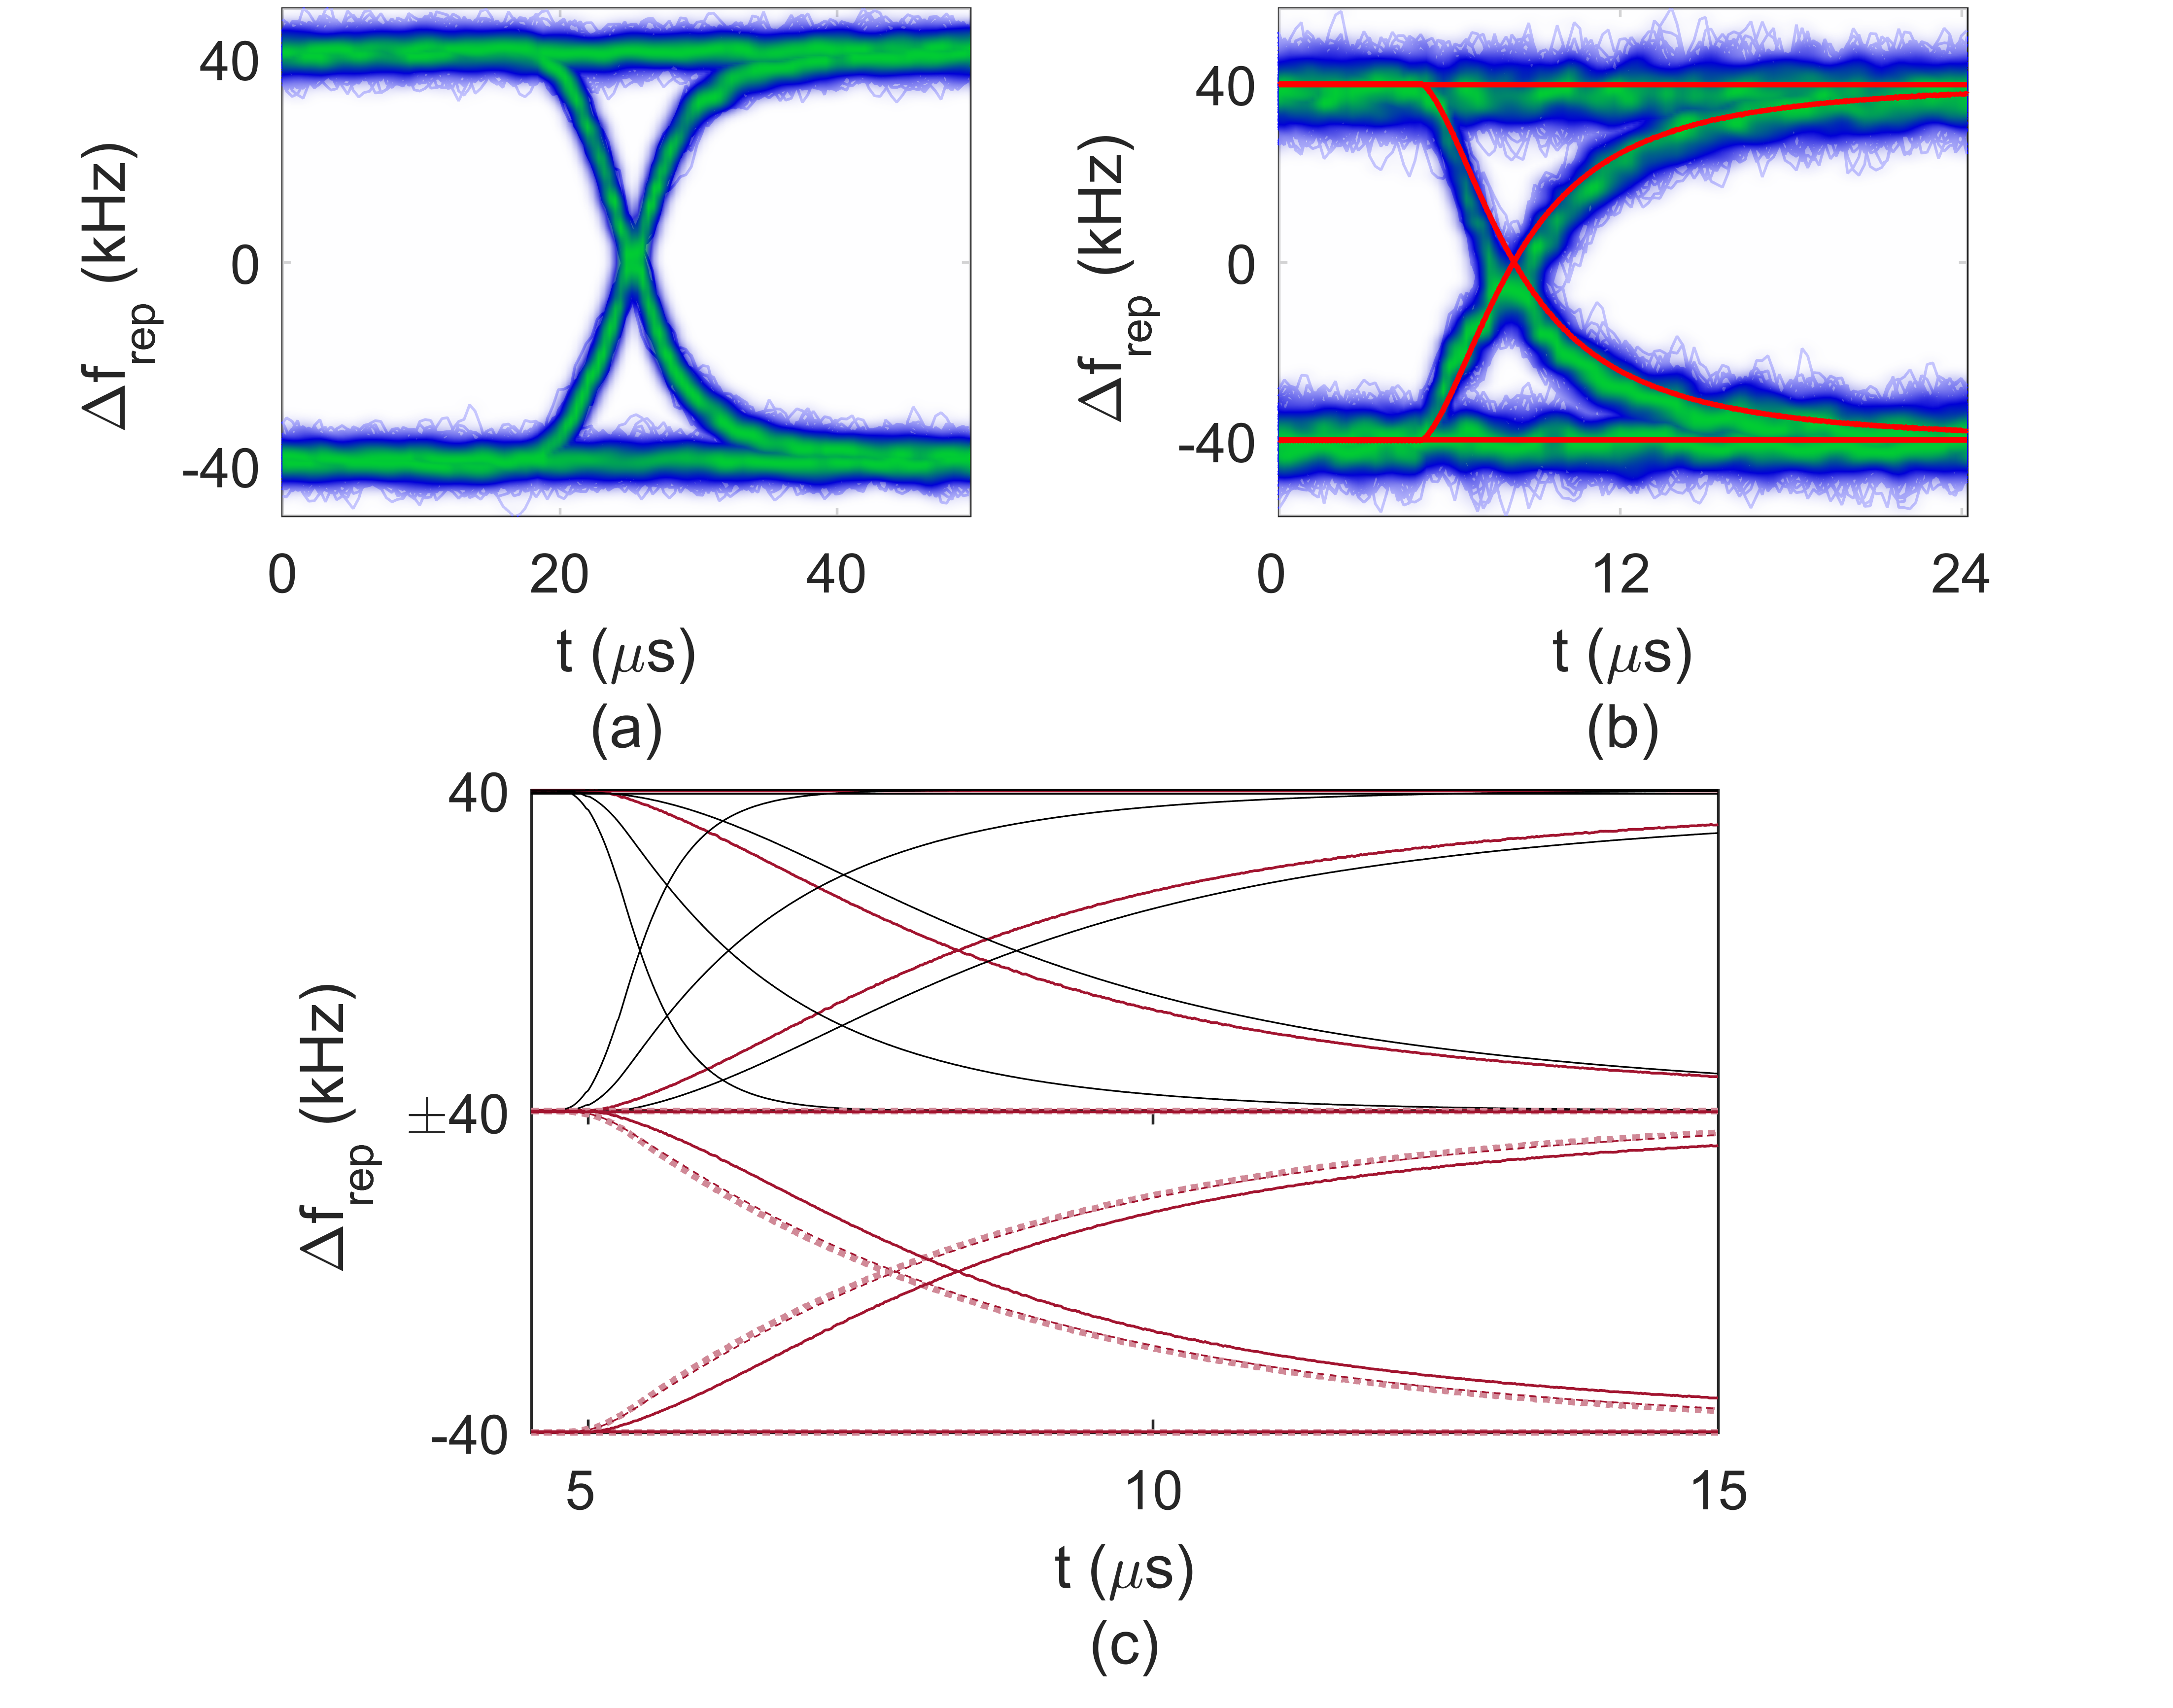
\includegraphics{\FigPath/Figures/PMPumping/PMeyediags.png}
	\end{center}
	\caption[Repetition-rate switching driven by a phase-modulated pump laser]{\textbf{Repetition-rate switching driven by a phase-modulated pump laser.} (a) Measured eye-diagram showing the switching capability of the soliton pulse train's repetition rate as $f_{PM}$ is switched over $\pm$40 kHz with 10 $\mu$s transition time. (b) The same with 60 ns transition time, with an LLE simulation of the dynamics (red) overlaid. The simulation parameters are $\delta_{PM}=0.9\pi$, $\Delta\nu=1.5$ MHz. (c) Simulated switching dynamics for various linewidths and modulation depths. Top: $\Delta\nu$=10 MHz (fastest, left), 3 MHz, and 1.4 MHz (traces shown in solid black). Bottom: depths of $2\pi$ and $6\pi$ (dashed red, curves nearly overlap). In each, the other parameter matches the simulation in (c), which is shown again in solid red. }
	\label{fig:PMeyediags}
\end{figure} 

To evaluate the utility of phase modulation for fast control of the soliton's properties, we measure the repetition rate of the pulse train as $f_{PM}$ is rapidly switched by $\pm$40 kHz, which is within the soliton's locking range.  To measure these fast dynamics, we split the photodetected repetition-rate signal and send one path through a reactive circuit element (a set of low-pass filters) that induces a frequency-dependent phase shift. By comparing the phase between the two paths as a function of time, the time-dependent repetition rate can be determined. We construct eye-diagrams out of the resulting data; these are shown in Fig. \ref{fig:PMeyediags}. In Fig. \ref{fig:PMeyediags}a, $f_{PM}$ is switched with 200 $\mu$s period and 10 $\mu$s transition time; in Fig. \ref{fig:PMeyediags}b it is switched with 100 $\mu$s period and 60 ns transition time. These eye diagrams show that the PM enables exquisite control of the soliton pulse train.

We overlay a simulated eye diagram on the data in Fig. \ref{fig:PMeyediags}b. This simulation is conducted for parameters $\Delta\nu=1.5$ MHz, $\delta_{PM}=0.9\pi$ that are near the experimental values, and the agreement between measurement and simulation indicates that the measurements are consistent with fundamental LLE dynamics. Fig. \ref{fig:PMeyediags}c presents the results of additional LLE simulations; the basic result is that the switching speed of $f_{rep}$ is limited by the resonator linewidth, and can be only modestly improved by increasing $\delta_{PM}$. 



\section{Subharmonic phase modulation for high repetition-rate systems}

One apparent barrier to the use of a phase-modulated pump laser for single-soliton generation and manipulation is the electronically-inaccessible FSRs of some typical microcomb resonators. However, it is possible to overcome this challenge by phase modulating at a subharmonic of the FSR.  Simulations indicate that PM can directly excite single solitons with small modulation depth, e.g. $\delta_{PM}=0.15\pi$. In this limit, only the first-order PM sidebands are relevant, and their amplitude and phase relative to the carrier control the dynamics. For a small desired modulation depth defined by the relationship between the first-order sidebands and the carrier, it is possible to modulate at a frequency $f_{PM}\sim f_{FSR}/N$ so that the $N$\textsuperscript{th}-order PM sidebands and the carrier address resonator modes with relative mode numbers -1, 0, and 1. The depth of modulation at the frequency $f_{PM}$ can be chosen to fix the amplitudes of the $N$\textsuperscript{th}-order PM sidebands relative to the carrier and target a desired effective modulation depth. It is worth noting that when N is odd, phase modulation is recovered when the sidebands of order $-N$, 0, and $N$ address resonator modes -1, 0, and 1. When $N$ is even the result is pure amplitude modulation, such that the driving term takes the form $F(1+A \cos{\theta})$. Simulations indicate that this AM profile also enables spontaneous single-soliton generation under some circumstances, but we note that this modulation profile cannot be obtained from a standard Mach-Zehnder modulator, which provides a drive like $F \cos(\eta+\delta \cos{\theta})$; AM in general may be less useful than PM because schemes of comparable complexity do not always provide robust trapping of solitons to the same point in the co-moving frame at which they are generated \cite{Hendry2018}.

\begin{figure}[htpb]
	\begin{center}
		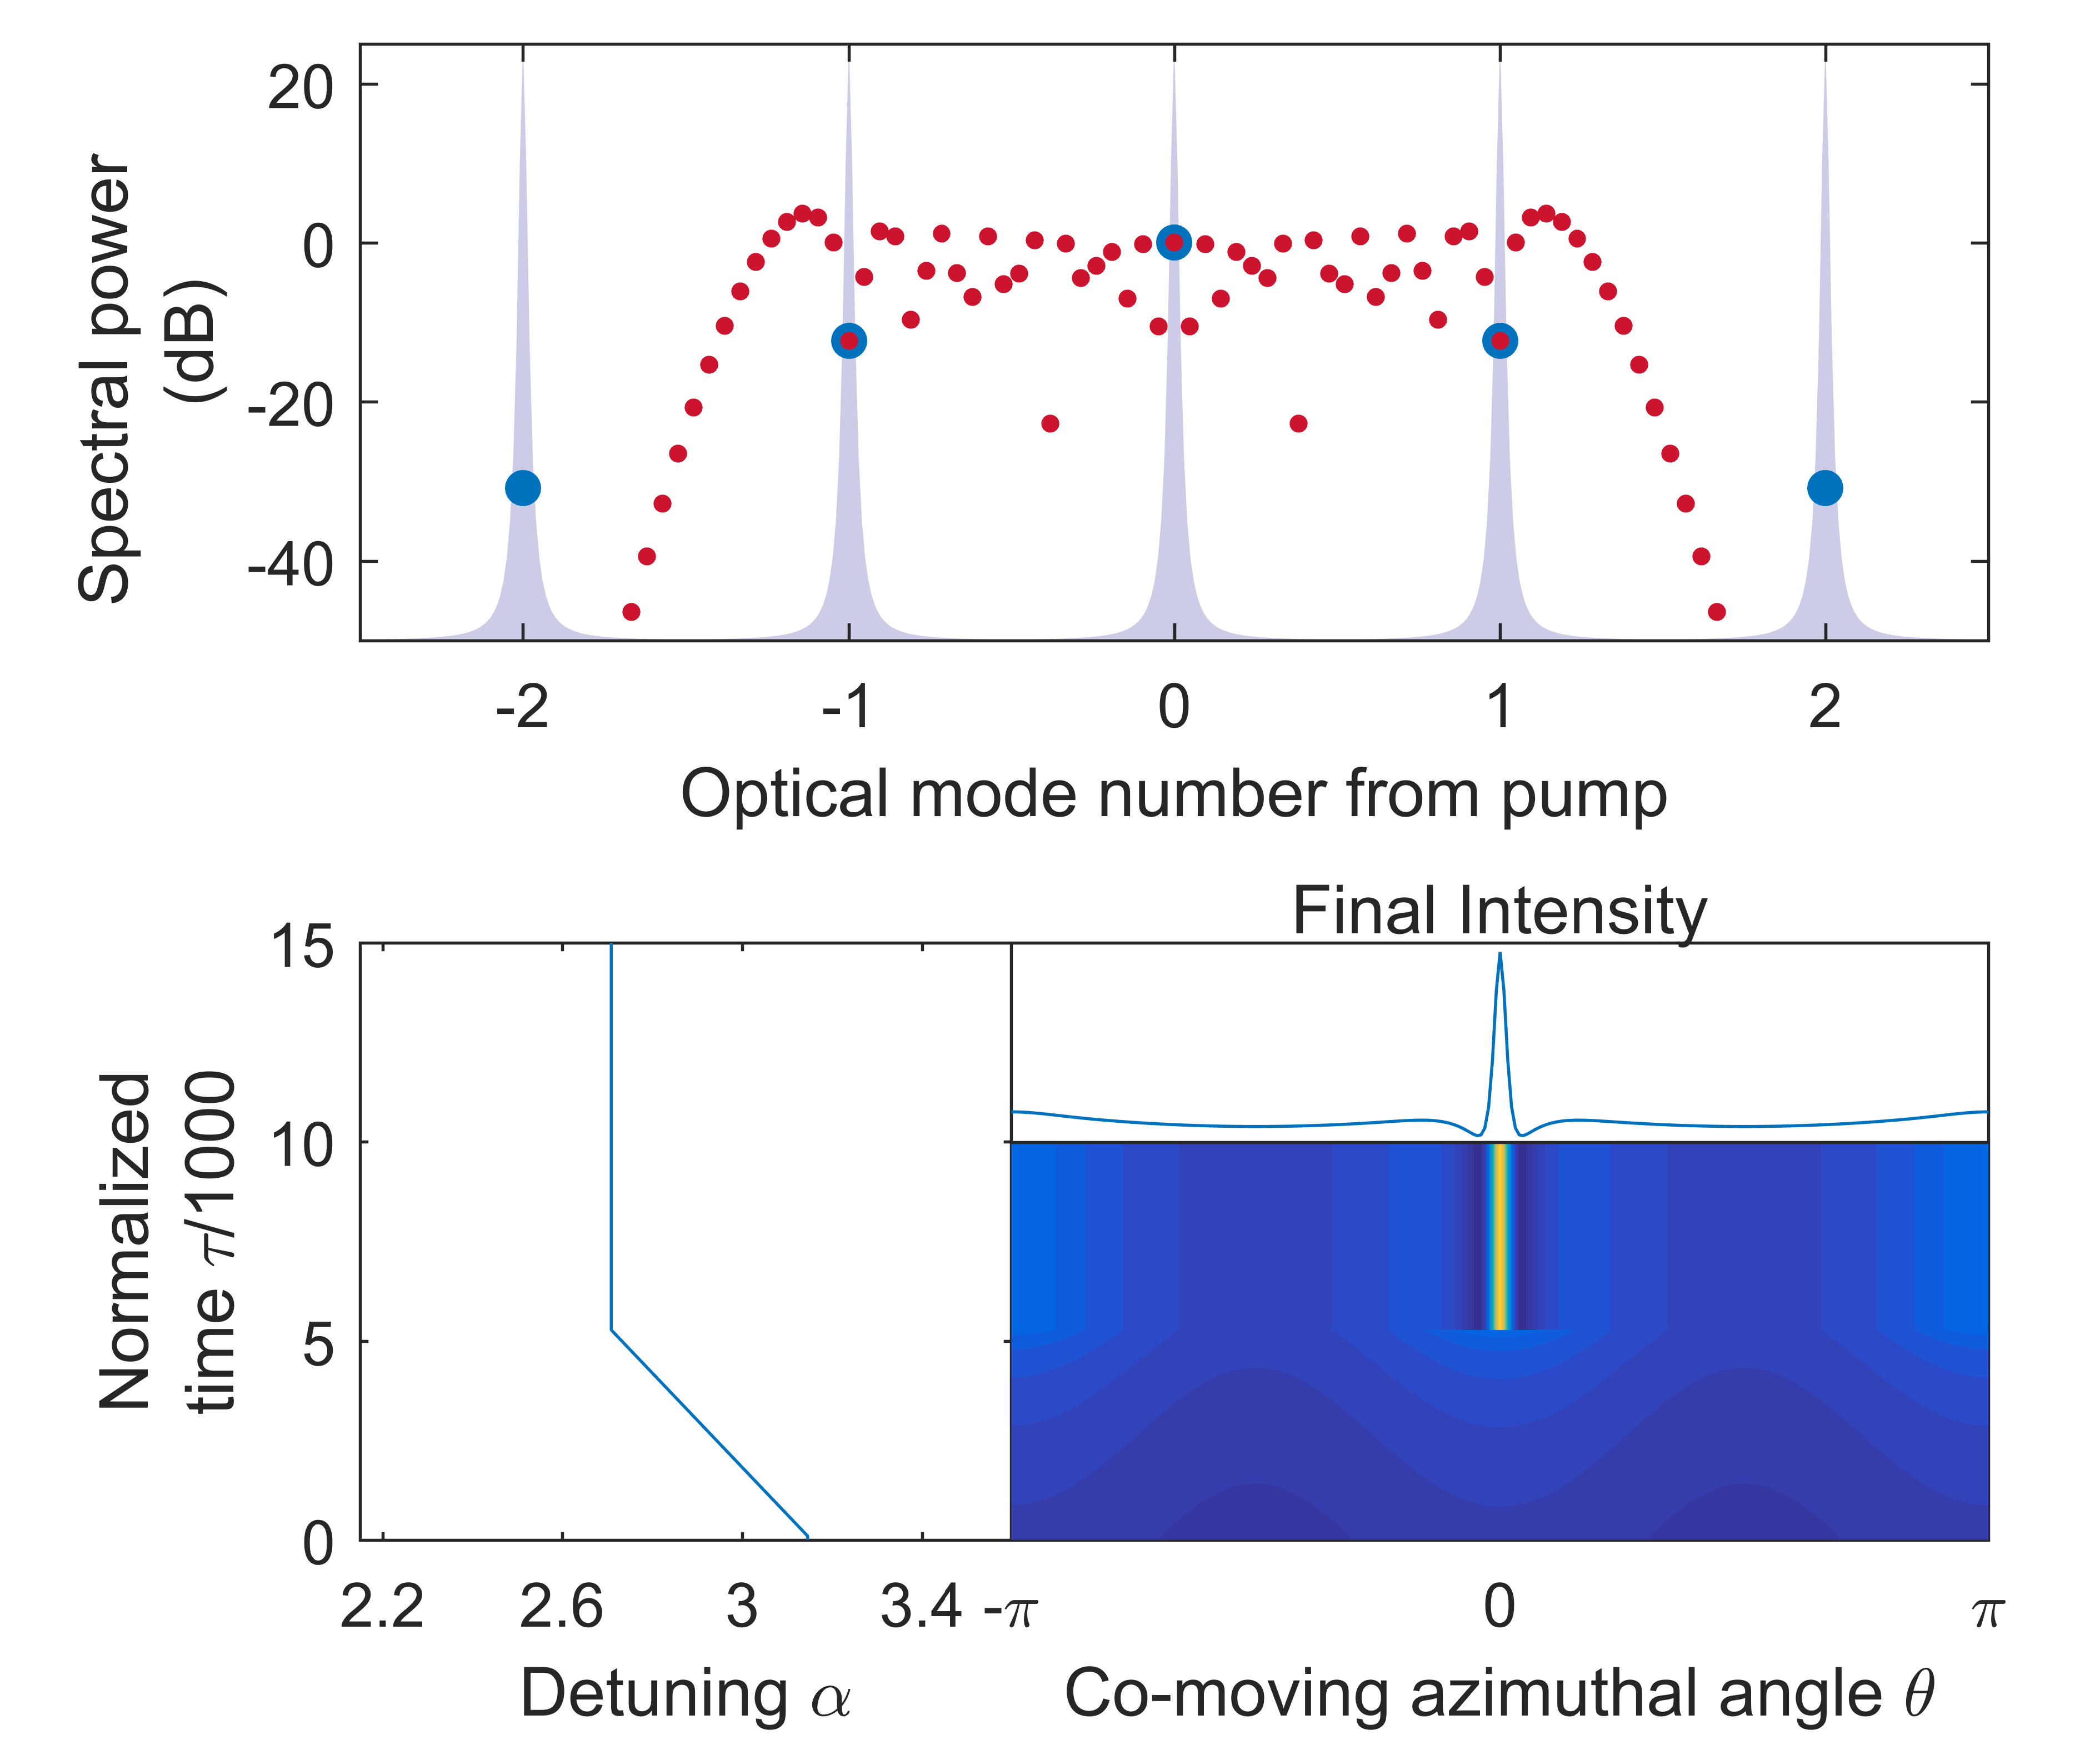
\includegraphics{\FigPath/Figures/PMPumping/PMsubharmonic.png}
	\end{center}
	\caption[Subharmonic phase modulation for high repetition-rate soliton generation]{\textbf{Subharmonic phase modulation for high-repetition-rate soliton generation.} (a) Spectra of PM at $f_{FSR}$ with depth $0.15\pi$ (blue) and at $f_{FSR}/21$ with depth $\sim$8.3$\pi$ (red). The relationships between the fields that address resonator mode numbers -1, 0, and 1 (as indicated by the gray Lorentzian curves) are the same in both cases. (b) LLE simulation of single-soliton generation using the subharmonic phase-modulation spectrum shown in red in panel (a). Only modes $n=0$, $\pm$21, $\pm$42,... of the phase-modulated driving field are coupled into the resonator and affect the LLE dynamics, with modes $|n|>$21 having negligible power. As $\alpha$ is increased from a large initial value, a soliton is spontaneously generated, exactly as in the case of phase modulation near the FSR.}
	\label{fig:PMsubharmonic}
\end{figure} 

Fig. \ref{fig:PMsubharmonic} presents an example of this technique. We simulate spontaneous soliton generation with PM at $f_{PM}=f_{rep}/N=f_{rep}/21$. The effective modulation depth is $0.15\pi$, which requires real modulation depth at the frequency $f_{PM}$ with depth $\delta_{PM}\sim8.3\pi$.  Because the phase modulation spreads the optical power into the PM sidebands, use of this technique requires higher optical power for the same effective pumping strength; in this example the optical power must be increased by $\sim$15.6 dB. A smaller real modulation depth could have been chosen to recover effective depth of $\delta_{eff}=0.15\pi$, but our chosen depth of $\sim8.3\pi$ gives better efficiency due to the higher ratio of the power in modes $0$, $\pm$21 to the total power in the spectrum. While the required modulation depth and pump power are higher with subharmonic phase modulation, neither is impractical. This technique could be used for spontaneous single-soliton generation in high-repetition rate systems; the example above indicates that it could be immediately applied in a 630 GHz-FSR resonator with 30 GHz phase modulation. 





%
%We demonstrate protected single-soliton formation and operation in a Kerr microresonator using a phase-modulated pump laser. Phase modulation gives rise to phase and amplitude variations in the resonator background, which in turn lead to an operation regime in which multi-soliton degeneracy is lifted and a single soliton is the only observable behavior. Direct excitation of single solitons is indicated by observed reversal of the characteristic ‘soliton step.’ Phase modulation also enables precise control of the soliton pulse train’s properties, and measured dynamics agree closely with simulations. We show that the technique can be extended to high repetition-frequency Kerr solitons through subharmonic phase modulation. These results facilitate straightforward generation and control of Kerr-soliton microcombs in integrated photonics systems. 
%
%
%
%Dissipative temporal cavity solitons in Kerr microresonators [1–3] have the potential to provide the revolutionary capabilities of frequency combs in a chip-integrable platform. This would extend the reach of frequency combs to applications in communications,  computation, and sensing with low size, weight, and power. Progress has come rapidly in the field of microresonator-soliton-based frequency combs, but for these combs to reach applications, simple, repeatable, and platform-independent methods of soliton generation and control are needed. The basic challenge is that solitons in microresonators are independent excitations, and a resonator can host zero, one, or many co-circulating solitons at a given pump-laser power and frequency, with each soliton giving rise to its own out-coupled pulse train. Further, under normal conditions solitons can only be generated by condensation from extended modulation-instability (MI) patterns (primary comb/Turing patterns, or noisy comb/spatiotemporal chaos) that provide appropriate initial conditions. Thermal stability must be maintained during the drop in intracavity power associated with the transition from a high duty-cycle MI pattern to a low duty-cycle soliton. A variety of schemes have been demonstrated to address these challenges and obtain single solitons [4–7], and many achieve excellent performance. In general these schemes increase experimental complexity, exploiting non-adiabatic variations in pump-laser power and frequency, and involve at least some amount of stochastic fluctuation in the output. 
%One notable possibility is modulation of the pump laser at a frequency near the resonator free-spectral range (FSR) [8–11], which can enable deterministic condensation of either one or zero solitons from an MI pattern. Further, it has been demonstrated that phase modulation (PM) can facilitate generation and control of single solitons [10,12,13]. Here we use PM at the FSR to deterministically excite single solitons directly from a chirped background that is stable elsewhere, as proposed in Ref.  [14]. Exiting the resonator is a train of solitons spaced by the round-trip time, as shown in Fig. 1a.  Importantly, no transient perturbation to the system parameters is required.
%Our results demonstrate a regime in which single-soliton operation is fundamentally protected, without the degeneracy between N=0,1, and many solitons that exists for a continuous-wave (CW) pump laser.  To motivate the experimental work that follows, we present theoretical results that illustrate the utility of a PM pump. We use the nonlinear partial-differential Lugiato-Lefever equation (LLE) with modification of the driving term for phase-modulation of depth δ_PM [1,14–17]:
%
%
%The normalized quantities used in the LLE are defined as follows [15]: ψ is the envelope for the intracavity field normalized so that |ψ|^2=1 at the absolute threshold for parametric oscillation; τ=t/2τ_γ, where t is the time and τ_γ=1/2πΔν is the cavity photon lifetime and Δν is the cavity resonance linewidth; α=2(ν_0-ν_pump )/Δν is the detuning between the pumped resonance with frequency ν_0 and the pump laser with frequency ν_pump; F is the pump strength normalized so that F^2=1 at the absolute threshold for parametric oscillation; and β_2=-2D_2/Δν<0 is the anomalous resonator dispersion, with D_2/2π=∂^2 ν_μ/∂μ^2 |_(μ=0)>0, where ν_μ represents the set of cavity resonance frequencies. The azimuthal angle θ co-rotates at the frequency f_PM, which is presently assumed to be equal to f_FSR.
%
%
%We perform simulations of the LLE to investigate soliton degeneracy for the range of pump-laser detunings overwhich solitons exist. These simulations use a fourth-order Runge-Kutta algorithm in the interaction picture [18] with adaptive step size [19]. A comparison of the resulting soliton energy-level diagrams for the CW case (δ_PM=0) and the PM case (δ_PM=π/2) are shown in Fig. 1b. We find that PM transforms the resonator excitation spectrum from a series of N=0,1,2,…,N_max solitons to a single level N=1 near threshold, eliminating degeneracy between these states. This occurs due to amplitude variations resulting from the phase modulation, with dispersion and nonlinearity providing PM-to-AM conversion. We can gain some insight into the origin of this effect by inserting the ansatz ψ(θ,τ)=ϕ(θ,τ)e^(iδ_PM  cos⁡θ ) into Eq. (1) [13].  By expanding the second-derivative term and setting derivatives of ϕ to zero we arrive at an equation for the quasi-CW background in the PM-pumped resonator:
%F=(γ(θ)+iα_eff (θ))ϕ-i|ϕ|^2 ϕ,	(2)
%where we have defined effective loss and detuning terms:
%γ(θ)=1+β_2/2 δ_PM  cos⁡θ,	(3)
%α_eff (θ)=α-β_2/2 δ_PM^2  sin^2⁡θ.	(4)
%
%
%
%
%
%This equation yields an approximate solution for ψ:
%ψ=(Fe^(iδ_PM  cos⁡θ ))/(γ(θ)+i(α_eff (θ)-ρ(θ)) ),	(5)
%where ρ(θ)=|ϕ(θ)|^2 is the (smallest real) solution to the cubic polynomial in ρ that results from calculating the modulus-square of Eq. (2). In neglecting the spatial derivatives of ϕ but retaining the derivatives of the phase term e^(iδ_PM  cos⁡θ ) we have made the approximation that the dominant effect of dispersion comes from its action on the existing broadband phase-modulation spectrum. This model reveals that amplitude variations in the quasi-CW background can be expected as a result of the spatially-varying effective loss and detuning terms that arise from the periodically-chirped pump laser.
%Fig. 1c compares the predictions of numerical LLE simulations (color) with the analytical model (black). The two agree quantitatively at small modulation depth (δ_PM=π/2, blue) and qualitatively at larger depth (δ_PM=4π, green). Both the simulations and the approximate analytic solution indicate that the background has two peaks per round trip in the presence of phase modulation, which suggests a mechanism for spontaneous single-soliton generation: At threshold the larger peak becomes locally unstable, and a soliton forms [20,21]. Moreover, it is known that if solitons exist elsewhere they are pushed to the larger peak by the background’s modulated phase [13]. This makes superpositions of N>1 solitons unstable and practically forbidden. Generation of single solitons then simply requires tuning the pump power and frequency to appropriate values, regardless of initial conditions. 
%The detuning for soliton generation can be estimated using Eq. (2) by calculating the value of α where ρ(θ=0)=1. This comes with a further approximation—simulations reveal that the critical detuning for soliton formation is near but not necessarily at ρ=1 because the spatial interval over which threshold is exceeded must have some minimum width. However, this approach quantitatively captures the behavior shown in Fig. 1b, predicting soliton generation at α=2.737.
%Because it is background intensity variations that result local MI and spontaneous soliton generation, it is natural to consider whether a similar technique can be employed using amplitude modulation (AM). In principle this can be done. However, to experimentally realize the robust single-soliton operation we describe below, the intensity modulation would need to yield a narrow cavity intensity maximum, and would therefore necessarily be broadband (e.g. pulsed pumping [11,21]), or would require supplementary PM to generate a trapping site for solitons. We are unaware of a straightforward implementation of AM for protected single-soliton operation that rivals the simplicity of the scheme presented here.
%We implement the approach described above to realize completely deterministic generation of single solitons without condensation from an extended pattern, summarized in Fig. 2. We use a 22 GHz-FSR silica ring resonator with Δν~1.5 MHz linewidth [22], pumped by a laser with normalized power F^2 between 2 and 6 that is phase-modulated at a rate f_PM~22 GHz with relatively small depth δ_PM~π. We overcome thermal instabilities [23] and control the detuning ν_0-ν_pump in real time using a frequency-agile pump [24], with an AOM-shifted probe for continuously monitoring the detuning. We decrease the detuning from a large initial value (~40 MHz), and a soliton is generated near 5 MHz (dependent upon the pump power and coupling condition). Measuring the power converted through FWM to new frequencies, the ‘comb power,’ reveals a step upon soliton formation, shown in Fig. 2a. This represents a reversal of the characteristic ‘soliton step’ that typically signals condensation of solitons from an extended pattern and indicates direct generation of a soliton from the background. After soliton generation, α may be increased again without loss of the soliton, consistent with Fig. 1b. We have verified that it is possible to turn off the PM while preserving the soliton (see also Ref.  [14]). 
%
%
%
%Automating soliton generation by repeatedly scanning the laser into resonance (detuning ~5 MHz) and back out again (20 MHz, far enough that the soliton is lost) has enabled reversible generation of 1000 solitons in 1000 trials over 100 seconds, with a 100 % measured success rate. Our probe-laser setup enables measurement of the detuning at which soliton generation occurs, which changes little from run to run. Fig. 2c presents a histogram of measurements for the generation of 160 solitons.
%Besides enabling protected sigle-soliton operation, PM pumping  also naturally provides timing and repetition-rate control, because the solitons are pushed towards the intracavity phase maximum [13]. This is illustrated in Fig. 3. In our experiments, the repetition rate of the out- coupled pulse train (f_rep) remains locked to f_PM over a bandwidth of ~±40 kHz. In Fig. 3a, we show a measured spectrogram of f_rep as f_PM  is swept sinusoidally over ±50 kHz. The repetition rate follows the PM except for glitches near the peaks of the sweep. In the inset of Fig. 3a we overlay the results of LLE simulations (see below) that qualitatively match the observed behavior. These simulations indicate that the periodic nature of the glitches is due to the residual pulling of the phase modulation on the soliton when the latter periodically cycles through the pump’s phase maximum. Our observed locking range of ~±40 kHz agrees well with an estimate δ_PM×D_2/2π~44 kHz [13] using the approximate measured value D_2=14 kHz per mode.
%Measured eye diagrams presented in Figs. 3b and 3c illustrate the switching of f_rep as f_PM is switched by 80 kHz around the soliton’s natural repetition rate. In Fig. 3b, f_PM is switched with 200 μs period and 10 μs transition time; in Fig. 3c it is switched with 100 μs period and 60 ns transition time. This data is obtained by detecting f_rep and passing the signal through two paths, one with an element that induces a frequency-dependent phase shift. From the resulting phase difference the repetition rate can be measured in real time. These eye diagrams show that the PM enables exquisite control of the soliton pulse train.
%We further explore the dynamics of repetition-rate switching by performing additional LLE simulations. We introduce the term +β_1  ∂ψ/∂θ to the right-hand side of Eq. (1), where β_1=-2(FSR-f_PM)/Δν represents a difference between the modulation frequency and the FSR 
%
%
%
%of the resonator near the pump wavelength [13,14];  β_1 may be varied in time.  In Fig. 3c we overlay a simulation of switching conducted for parameters (Δν=1.5 MHz, δ_PM=0.9 π) near the experimental values, and the agreement between measurements and simulation indicates that the measurements are consistent with fundamental LLE dynamics. We present the results of additional simulations in Fig. 3d; the basic observation is that the switching speed of f_rep is limited by the resonator linewidth, and can be modestly improved by increasing δ_PM.
%One apparent barrier to the use of a phase-modulated pump laser for protected single-soliton generation and manipulation is the electronically-inaccessible FSRs of some typical microcomb resonators. However, it is possible to overcome this challenge by phase modulating at a subharmonic of the FSR.  Simulations indicate that PM can directly excite single solitons with small modulation depth, e.g. δ_PM=0.15π. In this limit, only the first-order PM sidebands are relevant, and their amplitude and phase relative to the carrier control the dynamics. For a small desired modulation depth defined by the relationship between the first-order sidebands and the carrier, it is possible to modulate
%
%
%at a frequency ~f_FSR/N so that the N^th-order PM sidebands and the carrier address resonator modes with relative mode numbers -1, 0, and 1. The depth of modulation at the frequency f_FSR/N can be chosen to fix the amplitudes of the N^th-order PM sidebands relative to the carrier and target a desired effective modulation depth. It is worth noting that when N is odd, phase modulation is recovered when the sidebands of order -N,0, and N address resonator modes -1, 0, and 1. When N is even the result is pure amplitude modulation, such that the driving term takes the form F(1+A cos⁡θ). Under some circumstances this AM profile also enables spontaneous single-soliton generation, but we note that this modulation profile cannot be obtained from a standard Mach-Zehnder modulator, which provides a drive like F cos⁡(η+δ cos⁡θ ).
%Fig. 4 presents an example of this technique. We simulate protected single-soliton generation with PM at f_mod=f_rep/N=f_rep/21. The effective modulation depth is 0.15π, which requires real modulation depth at the frequency f_mod with depth δ_PM~8.3π.  Because the phase modulation spreads the optical power into the PM sidebands, use of this technique requires higher optical power for the same effective pumping strength; in this example the optical power must be increased by ~15.6 dB. While the required modulation depth and pump power are higher with subharmonic phase modulation, neither is impractical. This technique could be used for protected single-soliton generation in high-repetition rate systems; the example above indicates that it could be immediately applied to deterministic single-soliton generation in a 630 GHz-FSR resonator with 30 GHz phase modulation. 
%In this work, we have shown that PM-pumping fundamentally changes a resonator’s excitation spectrum and enables a new regime of protected single-soliton operation. The technique is applicable to resonators with electronically accessible f_rep, which are important components of proposals for photonic integration of Kerr-solitons  [25,26], and can reach higher repetition-rate systems via subharmonic modulation. After soliton generation, the PM can optionally be turned off, recovering the properties of the non-PM soliton. We expect this technique to enable new experiments. For example, PM-pumped solitons are generated with known absolute timing, enabling immediate transduction of the modulation phase onto
%
%
%
%
%the pulse train; this is impossible with solitons stochastically condensed from an extended pattern. Our work brings microresonator solitons closer to applications.
